%\documentclass[hyperref={pdfpagelabels=false},slidetop,9pt]{beamer}
\documentclass[slidetop,8pt]{beamer}
\usepackage[T1]{fontenc}
\usepackage[utf8]{inputenc}
\newcommand{\id}{71}
\newcommand{\nom}{Théorie des mécanismes}
\newcommand{\sequence}{04}
\newcommand{\nomsequence}{Liaisons entre les solides}
\newcommand{\num}{02}
\newcommand{\type}{KH}
\newcommand{\descrip}{Liaisons équivalentes, hyperstatisme, liaisons en série et en parallèle, théorie des graphes}
\newcommand{\competences}{B2-12: Proposer une modélisation des liaisons avec leurs caractéristiques géométriques. \\ &  B2-13: Proposer un modèle cinématique paramétré à partir d'un système réel, d'une maquette numérique ou d'u \\ &  B2-17: Simplifier un modèle de mécanisme. \\ &  B2-18: Modifier un modèle pour le rendre isostatique. \\ &  C1-04: Proposer une démarche permettant d'obtenir une loi entrée-sortie géométrique.  \\ &  C2-05: Caractériser le mouvement d'un repère par rapport à un autre repère. \\ &  C2-06: Déterminer les relations entre les grandeurs géométriques ou cinématiques. }
\newcommand{\nbcomp}{7}
\newcommand{\systemes}{}
\newcommand{\systemesnum}{}
\newcommand{\systemessansaccent}{}
\newcommand{\ilot}{2}
\newcommand{\ilotstr}{02}
\newcommand{\dossierilot}{\detokenize{Ilot_02 }}

\usepackage{etex}
\usepackage{tikz}
\usepackage[european]{circuitikz}
\usepackage{pgf}
\usepackage[all]{xy}
\usepackage{pgfpages}
\usepackage{graphbox}
\usepackage{pdfpages}
%\usepackage[adobe-utopia]{mathdesign}
\usepackage{ifthen}
\usepackage{cancel}
\usepackage{framed}
\usepackage{subfig}
\usepackage{tabularx}
\usepackage{setspace}
\usepackage{soul}
\usepackage{schemabloc}
\usepackage{eqnarray}
\usepackage[dot, phantomtext]{dashundergaps}
\usepackage{media9}
\usepackage{multimedia}
\usepackage{textcomp}
\usefonttheme[onlymath]{serif}

\author{Renaud Costadoat}
\institute{Lycée Dorian}

\usepackage{multido}
\usepackage{multirow}
\usepackage{multicol} % Portions de texte en colonnes
\usepackage{flafter}%floatants après la référence

\usepackage{color}
\usepackage{xcolor}
\usepackage{colortbl}

\usepackage[gen]{eurosym}
\usepackage{tikz}
%\usepackage{pstricks,pst-node,pst-tree,pst-solides3d}
\usepackage{lmodern}
\usepackage[francais]{babel}
\usepackage{pslatex}
\usetheme{renaud}
\usepackage{times}
\usepackage[frenchmath]{newtxsf} % for sans serif symbols
\renewcommand{\familydefault}{\sfdefault}
%\usepackage{amsfonts}
%\usepackage{amsmath}
%\usepackage{mathastext}
\usepackage{verbatim}
\usepackage{moreverb}
%\usetikzlibrary{arrows,shapes}
\usepackage{graphicx}
\usepackage{psfrag}
\usepackage{wrapfig}
\usepackage{etoolbox}

\definecolor{gris25}{gray}{0.75}
\definecolor{bleu}{RGB}{18,33,98}
\definecolor{bleuf}{RGB}{42,94,171}
\definecolor{bleuc}{RGB}{231,239,247}
\definecolor{rougef}{RGB}{185,18,27}
\definecolor{rougec}{RGB}{255,188,204}%255,230,231
\definecolor{vertf}{RGB}{103,126,82}
\definecolor{vertc}{RGB}{220,255,191}

\setlength\parindent{24pt}
\parskip 7.2pt
\parindent 8pt

\newenvironment{rem}[1][\hsize]%
{%
    \def\FrameCommand
   {%
\rotatebox{90}{\textit{\textsf{Remarque}}} 
       {\color{bleuf}\vrule width 3pt}%
       \hspace{0pt}%must no space.
       \fboxsep=\FrameSep\colorbox{bleuc}%
  }%
    \MakeFramed{\hsize#1\advance\hsize-\width\FrameRestore}%
}%
{\endMakeFramed}%


\newenvironment{savoir}[1][\hsize]%
{%
    \def\FrameCommand
    {%
\rotatebox{90}{\textit{\textsf{Savoir}}} 
        {\color{bleuf}\vrule width 3pt}%
        \hspace{0pt}%must no space.
        \fboxsep=\FrameSep\colorbox{bleuc}%
    }%
    \MakeFramed{\hsize#1\advance\hsize-\width\FrameRestore}%
}%
{\endMakeFramed}%

\newenvironment{prob}[1][\hsize]%
{%
    \def\FrameCommand%
    {%
\rotatebox{90}{\textit{\textsf{Problematique}}} 
        {\color{rougef}\vrule width 3pt}%
        \hspace{0pt}%must no space.
        \fboxsep=\FrameSep\colorbox{rougec}%
    }%
    \MakeFramed{\hsize#1\advance\hsize-\width\FrameRestore}%
}%
{\endMakeFramed}%

\newenvironment{obj}[1][\hsize]%
{%
    \def\FrameCommand%
    {%
\rotatebox{90}{\textit{\textsf{Objectif}}} 
        {\color{vertf}\vrule width 3pt}%
        \hspace{0pt}%must no space.
        \fboxsep=\FrameSep\colorbox{vertc}%
    }%
    \MakeFramed{\hsize#1\advance\hsize-\width\FrameRestore}%
}%
{\endMakeFramed}%

\newenvironment{defi}[1][\hsize]%
{%
    \def\FrameCommand%
    {%
\rotatebox{90}{\textit{\textsf{Definition}}} 
        {\color{bleuf}\vrule width 3pt}%
        \hspace{0pt}%must no space.
        \fboxsep=\FrameSep\colorbox{rougec}%
    }%
    \MakeFramed{\hsize#1\advance\hsize-\width\FrameRestore}%
}%
{\endMakeFramed}%


\newenvironment{hypo}[1][\hsize]%
{%
    \def\FrameCommand%
    {%
\rotatebox{90}{\textit{\textsf{Hypothèse\\}}} 
        {\color{bleuf}\vrule width 3pt}%
        \hspace{0pt}%must no space.
        \fboxsep=\FrameSep\colorbox{bleuc}%
    }%
    \MakeFramed{\hsize#1\advance\hsize-\width\FrameRestore}%
}%
{\endMakeFramed}%


\newenvironment{prop}[1][\hsize]%
{%
    \def\FrameCommand%
    {%
\rotatebox{90}{\textit{\textsf{Propriété}}} 
        {\color{bleuf}\vrule width 3pt}%
        \hspace{0pt}%must no space.
        \fboxsep=\FrameSep\colorbox{bleuc}%
    }%
    \MakeFramed{\hsize#1\advance\hsize-\width\FrameRestore}%
}%
{\endMakeFramed}%

\newenvironment{props}[1][\hsize]%
{%
    \def\FrameCommand%
    {%
\rotatebox{90}{\textit{\textsf{Propriétés}}} 
        {\color{bleuf}\vrule width 3pt}%
        \hspace{0pt}%must no space.
        \fboxsep=\FrameSep\colorbox{bleuc}%
    }%
    \MakeFramed{\hsize#1\advance\hsize-\width\FrameRestore}%
}%
{\endMakeFramed}%

\newenvironment{exemple}[1][\hsize]%
{%
    \def\FrameCommand%
    {%
\rotatebox{90}{\textit{\textsf{Exemple}}} 
        {\color{vertf}\vrule width 3pt}%
        \hspace{0pt}%must no space.
        \fboxsep=\FrameSep\colorbox{vertc}%
    }%
    \MakeFramed{\hsize#1\advance\hsize-\width\FrameRestore}%
}%
{\endMakeFramed}%

\newenvironment{resultat}[1][\hsize]%
{%
    \def\FrameCommand%
    {%
\rotatebox{90}{\textit{\textsf{Résultat}}} 
        {\color{rougef}\vrule width 3pt}%
%        {\color{bleuf}\vrule width 3pt}%
        \hspace{0pt}%must no space.
        \fboxsep=\FrameSep\colorbox{rougec}%
    }%
    \MakeFramed{\hsize#1\advance\hsize-\width\FrameRestore}%
}%
{\endMakeFramed}%

\newenvironment{methode}[1][\hsize]%
{%
    \def\FrameCommand%
    {%
\rotatebox{90}{\textit{\textsf{Méthode\\}}} 
        {\color{rougef}\vrule width 3pt}%
        \hspace{0pt}%must no space.
        \fboxsep=\FrameSep\colorbox{rougec}%
    }%
    \MakeFramed{\hsize#1\advance\hsize-\width\FrameRestore}%
}%
{\endMakeFramed}%

\newenvironment{theo}[1][\hsize]%
{%
    \def\FrameCommand%
    {%
\rotatebox{90}{\textit{\textsf{Théorème\\}}} 
        {\color{rougef}\vrule width 3pt}%
        \hspace{0pt}%must no space.
        \fboxsep=\FrameSep\colorbox{rougec}%
    }%
    \MakeFramed{\hsize#1\advance\hsize-\width\FrameRestore}%
}%
{\endMakeFramed}%

\newenvironment{warn}[1][\hsize]%
{%
    \def\FrameCommand%
    {%
\rotatebox{90}{\textit{\textsf{Attention\\}}} 
        {\color{rougef}\vrule width 3pt}%
        \hspace{0pt}%must no space.
        \fboxsep=\FrameSep\colorbox{rougec}%
    }%
    \MakeFramed{\hsize#1\advance\hsize-\width\FrameRestore}%
}%
{\endMakeFramed}%

% \usepackage{pstricks}
%\usepackage{minitoc}
% \setcounter{minitocdepth}{4}

\setcounter{tocdepth}{2}

% \mtcselectlanguage{french} 

%\usepackage{draftcopy}% "Brouillon"
% \usepackage{floatflt}
\usepackage{psfrag}
%\usepackage{listings} % Permet d'insérer du code de programmation
\renewcommand{\baselinestretch}{1.2}

% Changer la num�rotation des figures :
% ------------------------------------
% \makeatletter
% \renewcommand{\thefigure}{\ifnum \c@section>\z@ \thesection.\fi
%  \@arabic\c@figure}
% \@addtoreset{figure}{section}
% \makeatother
 


%%%%%%%%%%%%
% Définition des vecteurs %
%%%%%%%%%%%%
 \newcommand{\vect}[1]{\overrightarrow{#1}}

%%%%%%%%%%%%
% Définition des torseusr %
%%%%%%%%%%%%

 \newcommand{\torseur}[1]{%
\left\{{#1}\right\}
}

\newcommand{\torseurcin}[3]{%
\left\{\mathcal{#1} \left(#2/#3 \right) \right\}
}

\newcommand{\torseurstat}[3]{%
\left\{\mathcal{#1} \left(#2\rightarrow #3 \right) \right\}
}

 \newcommand{\torseurc}[8]{%
%\left\{#1 \right\}=
\left\{
{#1}
\right\}
 = 
\left\{%
\begin{array}{cc}%
{#2} & {#5}\\%
{#3} & {#6}\\%
{#4} & {#7}\\%
\end{array}%
\right\}_{#8}%
}

 \newcommand{\torseurcol}[7]{
\left\{%
\begin{array}{cc}%
{#1} & {#4}\\%
{#2} & {#5}\\%
{#3} & {#6}\\%
\end{array}%
\right\}_{#7}%
}

 \newcommand{\torseurl}[3]{%
%\left\{\mathcal{#1}\right\}_{#2}=%
\left\{%
\begin{array}{l}%
{#1} \\%
{#2} %
\end{array}%
\right\}_{#3}%
}

 \newcommand{\vectv}[3]{%
\vect{V\left( {#1} \in {#2}/{#3}\right)}
}


\newcommand{\vectf}[2]{%
\vect{R\left( {#1} \rightarrow {#2}\right)}
}

\newcommand{\vectm}[3]{%
\vect{\mathcal{M}\left( {#1}, {#2} \rightarrow {#3}\right)}
}


 \newcommand{\vectg}[3]{%
\vect{\Gamma \left( {#1} \in {#2}/{#3}\right)}
}

 \newcommand{\vecto}[2]{%
\vect{\Omega\left( {#1}/{#2}\right)}
}

\newcommand{\reponse}[1][4]
{
\multido{}{#1}
{
\begin{center}
\makebox[0.9\linewidth]{\dotfill} \end{center}
}}


% }$$\left\{\mathcal{#1} \right\}_{#2} =%
% \left\{%
% \begin{array}{c}%
%  #3 \\%
%  #4 %
% \end{array}%
% \right\}_{#5}}


%  ------------------------------------------
% | Modification du formatage des sections : | 
%  ------------------------------------------

% Grands titres :
% ---------------

\newcommand{\titre}[1]{%
\begin{center}
      \bigskip
      \rule{\textwidth}{1pt}
      \par\vspace{0.1cm}
      
      \textbf{\large #1}
      \par\rule{\textwidth}{1pt}
    \end{center}
    \bigskip
  }

% Supprime le numéro du chapitre dans la numérotation des sections:
% -----------------------------------------------------------------
\makeatletter
\renewcommand{\thesection}{\@arabic\c@section}
\makeatother


% \titleformat{\chapter}[display]
% {\normalfont\Large\filcenter}
% {}
% {1pc}
% {\titlerule[1pt]
%   \vspace{1pc}%
%   \Huge}[\vspace{1ex}%
% \titlerule]


%%%% Chapitres Comme PY Pechard %%%%%%%%%
% numéro du chapitre
\DeclareFixedFont{\chapnumfont}{OT1}{phv}{b}{n}{80pt}
% pour le mot " Chapitre "
\DeclareFixedFont{\chapchapfont}{OT1}{phv}{m}{it}{40pt}
% pour le titre
\DeclareFixedFont{\chaptitfont}{T1}{phv}{b}{n}{25pt}

\definecolor{gris}{gray}{0.75}
\setbeamertemplate{section in toc}[sections numbered]

\newlength{\RoundedBoxWidth}
\newsavebox{\GrayRoundedBox}
\newenvironment{GrayBox}[1][\dimexpr\textwidth-4.5ex]%
   {\setlength{\RoundedBoxWidth}{\dimexpr#1}
    \begin{lrbox}{\GrayRoundedBox}
       \begin{minipage}{\RoundedBoxWidth}}%
   {   \end{minipage}
    \end{lrbox}
    \begin{center}
    \begin{tikzpicture}%
       \draw node[draw=bleuf,fill=bleuc,rounded corners,%
             inner sep=2ex,text width=\RoundedBoxWidth]%
             {\usebox{\GrayRoundedBox}};
    \end{tikzpicture}
    \end{center}}
    
\ifdef{\prive}{\pgfpagesuselayout{2 on 1}[a4paper,border shrink=0mm]}
\ifdef{\prive}{\setbeamertemplate{navigation symbols}{}}
\setbeamertemplate{itemize item}[ball]
%\setbeamertemplate{blocks}[rounded]%[shadow=true]
\setbeamercolor{block title}{fg=white,bg=grisf}        % titre block normal 
\setbeamercolor{block body}{fg=grisf,bg=grisc!50}      % corps block normal
\setbeamercolor{block body alerted}{fg=white,bg=warning}   % idem pour un block alerte

\title{\nom}
\date{S\sequence \ - \type\num}

\begin{document}
\shorthandoff{:!}
\bibliographystyle{abbrvnat-fr}

\usebackgroundtemplate%
{%
    \centering
\includegraphics[width=\paperwidth]{/home/renaud/Documents/Renaud/GitHub/Sciences-Ingenieur/img/fond2}%
}

{
\setbeamertemplate{navigation symbols}{}
\setbeamertemplate{headline}[pagetitre]
\setbeamertemplate{footline}[pagetitre]
\usebackgroundtemplate{\centering
\includegraphics[width=\paperwidth]{/home/renaud/Documents/Renaud/GitHub/Sciences-Ingenieur/img/fond}}
\frame{\titlepage}
}



{\frame{
\frametitle{Introduction}

\begin{savoir}
Vous êtes capables :
\begin{itemize}
 \item de modéliser un dipôle en fonction de ses caractéristiques,
 \item de manipuler des sources de tension et de courant,
 \item de modéliser un circuit et de déterminer ces caractéristiques grâce aux lois de l'électrocinétique.
\end{itemize}
\end{savoir}

\begin{prob}

Il est nécessaire d'utiliser d'autres formes de représentation d'un mécanisme.
\begin{itemize}
 \item \textit{Problème: Comment modéliser un convertisseur statique ?}
 \item \textbf{Perspectives}: Déterminer une méthode de modélisation et des critères de choix afin d'intégrer un convertisseur statique dans une chaîne d'énergie.
\end{itemize}
\end{prob}

}}

\section{Semi conducteurs de puissance} 
 
 
{\frame{
\frametitle{Interrupteurs à semi conducteurs}

L'électronique de puissance utilise des semi conducteurs fonctionnant en "interrupteurs". Les figures suivantes permettent de montrer le comportement d'un interrupteur.

\begin{minipage}{0.45\linewidth}
\begin{tikzpicture}
\fill [bleuc] (0,0) rectangle (1,-1);
\fill [bleuc] (0,0) rectangle (-1,1);
\draw[->] (-1.2,0) -- (1.2,0);
\draw (1.2,-0.4) node[above] {$v_k$};
\draw [->] (0,-1.2) -- (0,1.2);
\draw (0,1.2) node[right] {$i_k$};
\path (-0.1,-1) coordinate(src) ;
\path (0.1,1) coordinate(dst) ;
\path (-0.1,0.2) coordinate(ctrl1) ;
\path (0.1,-0.2) coordinate(ctrl2) ;
\draw[-, line width=1pt] (src) .. controls(ctrl1) and (ctrl2) .. (dst) ;
\path (-1,-0.1) coordinate(src2) ;
\path (1,0.1) coordinate(dst2) ;
\path (0.2,-0.1) coordinate(ctrl12) ;
\path (-0.2,0.1) coordinate(ctrl22) ;
\draw[-, line width=1pt] (src2) .. controls(ctrl12) and (ctrl22) .. (dst2) ;
\draw (0.1,1) node[right] {A};
\draw (1,0.1) node[above] {B};
\draw (-0.1,-1) node[left] {C};
\draw (-1,-0.1) node[below] {D};
\draw (-0.1,-0.1) node[below] {O};
%\node [draw,circle] at(0.7,0.7){1};
%\node [draw,circle] at(-0.7,-0.7){3};
\draw (0.5,-0.5) node[] {$\frac{v_k}{i_k}<0$};
\draw (-0.5,0.5) node[] {$\frac{v_k}{i_k}<0$};
\end{tikzpicture}
\end{minipage}
\hfill
\begin{minipage}{0.45\linewidth}
Un interrupteur équivaut à une résistance (toujours positive) :
\begin{itemize}
 \item très faible lorsqu'il est fermé,
 \item très forte lorsqu'il est ouvert.
\end{itemize}
\end{minipage}

}}

{\frame{
\frametitle{Définitions}

Un interrupteur idéal est considéré comme un \textbf{dipôle orienté} en convention \textbf{récepteur}.

\begin{minipage}{0.48\linewidth}
\centering\begin{circuitikz}
\draw[color=bleuf] 
(1,1) to[ospst=$K_1$, i=$i_k$] (3,1);
\draw (2.5,0.7) edge[-stealth] (1.3,0.7);	
\node (U) at (2,0.5){$v_k$};
\end{circuitikz}
\end{minipage}
\hfill
\begin{minipage}{0.48\linewidth}
\centering\begin{tikzpicture}
\draw[->] (-1.2,0) -- (1.2,0);
\draw (1.2,0) node[above] {$v_k$};
\draw [->] (0,-1.2) -- (0,1.2);
\draw (0,1.2) node[right] {$i_k$};
\draw[-, line width=2pt] (0,0) -- (1,0);
\draw[-, line width=2pt] (0,0) -- (0,1);
\draw (0.5,-0.5) node[] {Ouvert};
\draw (-0.5,0.5) node[] {Fermé};
\end{tikzpicture}
\end{minipage}

Il peut ainsi être caractérisé par les différents \textbf{segments} situés sur les axes du repère ($v_k$,$i_k$). Il existe alors des interrupteurs à 2, 3 ou 4 segments. Ils seront utilisés en fonction de besoins liés à la nature et aux réversibilités des \textbf{sources} et des \textbf{charges}. Il sera considéré que pour un interrupteur idéal, la caractéristique statique est \textbf{non dissipative}.
}}

{\frame{
\frametitle{Caractéristique dynamique}

La caractéristique \textbf{dynamique} d'un interrupteur est caractérisée par la trajectoire suivie par le point de fonctionnement pour passer d'un point situé sur un segment à un point situé sur un autre segment. Elle peut être amenée à passer dans un des quarts de plan ou suivre les axes comme on le verra plus loin.


L'étude de cette façon de commuter permet de prévoir les \textbf{pertes par commutation}. En effet, la puissance électrique est définie par: $P_{elec}=U.i$, celle ci est toujours positive (système dissipatif). Ainsi, deux cas de figure doivent être pris en compte:
\begin{itemize}
 \item Segments de signes opposés, le point de fonctionnement se déplace le long des axes: $W=0$ "commutation spontanée",
 \item Segments de même signe, déplacement dans un quart de plan : $W>0$ "commutation commandée à l'amorçage ou au blocage".
\end{itemize}

\begin{minipage}{0.48\linewidth}
\centering\begin{tikzpicture}
\draw[->] (-1.2,0) -- (1.2,0);
\draw (1.2,0) node[above] {$v_k$};
\draw [->] (0,-1.2) -- (0,0.5);
\draw (0,0.5) node[right] {$i_k$};
\draw[-] (1,0) -- (1,-0.1);
\draw[-] (0.1,-0.1) -- (1,-0.1);
\draw[-] (0.1,-0.1) -- (0.1,-0.6);
\draw[->] (0.1,-1) -- (0.1,-0.6);
\draw[-] (0,-1) -- (0.1,-1);
\draw[->] (0,0) -- (0,-0.4);
\draw (-1,-1.2) node[] {Spontanée};
\end{tikzpicture}
\end{minipage}
\hfill
\begin{minipage}{0.48\linewidth}
\centering\begin{tikzpicture}
\draw[->] (-1.2,0) -- (1.2,0);
\draw (1.2,0) node[above] {$v_k$};
\draw [->] (0,-0.5) -- (0,1.2);
\draw (0,1.2) node[right] {$i_k$};
\draw[-] (0,1) -- (1,1);
\draw[-] (0,0.9) -- (0.9,0.9);
\draw[->] (1,0) -- (1,0.6);
\draw[-] (1,0.6) -- (1,1);
\draw[->] (0.9,0.9) -- (0.9,0.4);
\draw[-] (0.9,0.4) -- (0.9,0);
\draw (-1,-0.5) node[] {Commandée};
\end{tikzpicture}
\end{minipage}


}}

{\frame{
\frametitle{Exemples d'interrupteurs}

Une \textbf{diode} est un interrupteur à 2 segments de signe opposés. Idéalement, elle ne peut donc commuter que sans pertes.

\begin{minipage}{.3\linewidth}
\centering\begin{circuitikz}
\draw[color=bleuf] 
(1,1) to[diode, i=$ik$] (3,1);
\draw (2.5,1.7) edge[-stealth] (1.3,1.7);	
\node (U) at (2,1.5){$U_{k}$};
\end{circuitikz}
\end{minipage}
\hfill
\begin{minipage}{.3\linewidth}
 \centering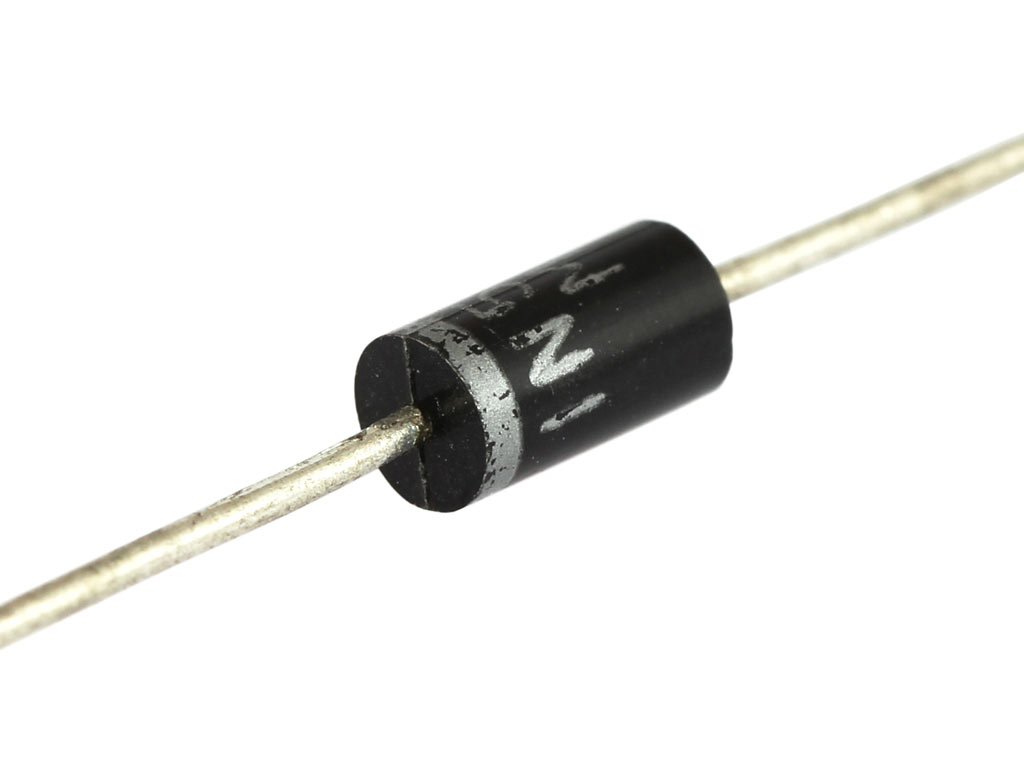
\includegraphics[width=0.8\linewidth]{img/diode}
\end{minipage}
\hfill
\begin{minipage}{.3\linewidth}
\centering\begin{tikzpicture}
\draw[->] (-1.2,0) -- (1.2,0);
\draw (1.2,0) node[above] {$v_k$};
\draw [->] (0,-0.5) -- (0,1.2);
\draw (0,1.2) node[right] {$i_k$};
\draw[-, line width=2pt] (-1.1,0) -- (0,0);
\draw[-, line width=2pt] (0,0) -- (0,1.1);
\draw[-, line width=1pt] (-1.1,0) -- (0.1,0);
\draw[-, line width=1pt] (0.1,0) -- (0.5,1.1);
\end{tikzpicture}
\end{minipage}


~\

Le \textbf{thyristor} est un interrupteur à 3 segments et à commande d'amorçage. La trajectoire du point de fonctionnement est représentée sur la figure suivante compte tenu de la présence de 2 segments de signe opposés.

\begin{minipage}{.3\linewidth}
\centering\begin{circuitikz}
\draw[color=bleuf] 
(1,1) to[thyristor, i=$ik$] (3,1);
\draw (2.5,1.7) edge[-stealth] (1.3,1.7);	
\node (U) at (2,1.5){$U_{k}$};
\end{circuitikz}
\end{minipage}
\hfill
\begin{minipage}{.3\linewidth}
 \centering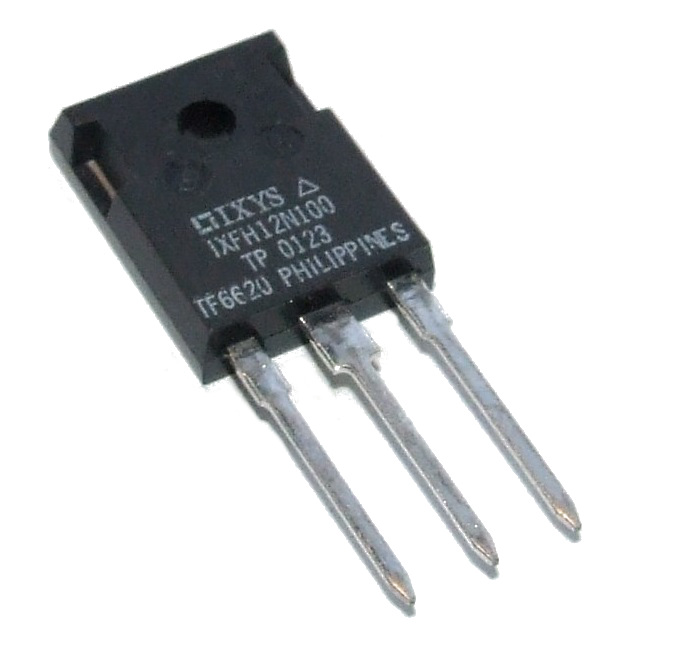
\includegraphics[width=0.8\linewidth]{img/thyristor}
\end{minipage}
\hfill
\begin{minipage}{.3\linewidth}
\centering\begin{tikzpicture}
\draw[->] (-1.2,0) -- (1.2,0);
\draw (1.2,0) node[above] {$v_k$};
\draw [->] (0,-0.5) -- (0,1.2);
\draw (0,1.2) node[right] {$i_k$};
\draw[-, line width=2pt] (-1.1,0) -- (1.1,0);
\draw[-, line width=2pt] (0,0) -- (0,1.1);
\draw[->] (1,1) -- (0.1,1);
\draw[-] (1,0) -- (1,1);
\draw[->] (-0.1,1) -- (-0.1,0.1);
\draw[->] (-0.1,0.1) -- (-1,0.1);
\draw[->] (-1,-0.1) -- (1,-0.1);
\draw (2,1) node[] {Commande};
\draw (2,0.5) node[] {d'amorçage};
\end{tikzpicture}
\end{minipage}
}}


{\frame{
\frametitle{Exemples d'interrupteurs}

L'\textbf{IGBT} est un interrupteur à 2 segments commandable à l'amorçage et au blocage.

\begin{minipage}{.3\linewidth}
\centering\begin{circuitikz} 
\draw[color=bleuf] (1,0) node[nigbt] (npn) {}
 (npn.base) node[anchor=east] {}
 (npn.collector) node[anchor=south] {}
 (npn.emitter) node[anchor=north] {};
 \draw[-,color=bleuf] (1,1) to[short, i=$ik$] (npn.collector);
 \draw (0,-1) edge[-stealth] (0,1);	
\node (U) at (-0.3,0){$U_{k}$};
\end{circuitikz}
\end{minipage}
\hfill
\begin{minipage}{.3\linewidth}
 \centering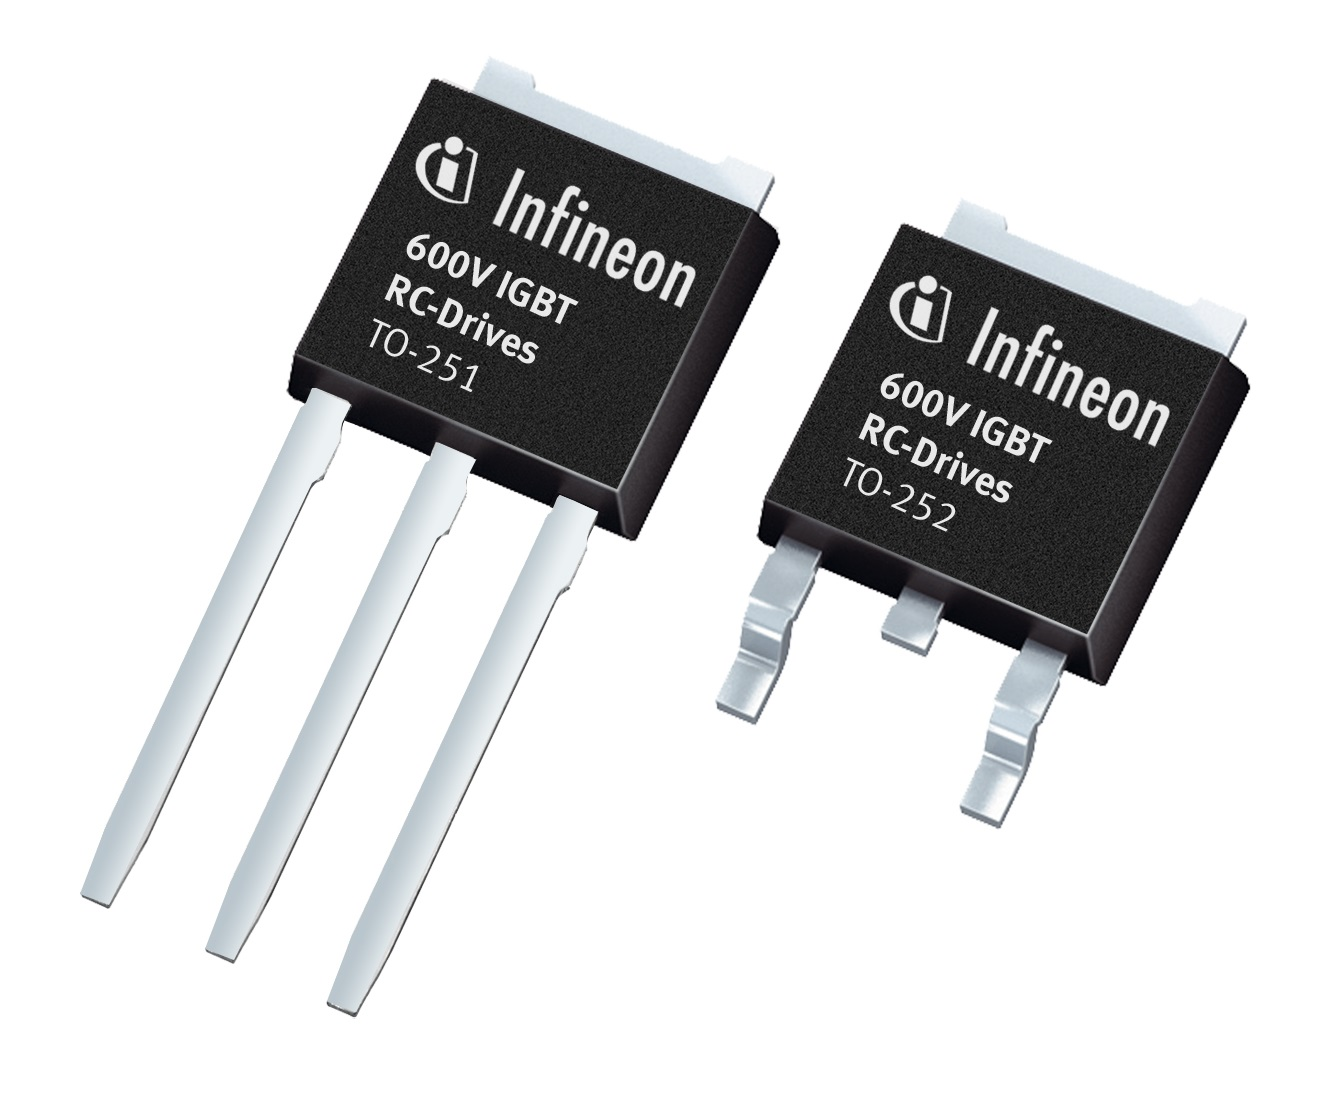
\includegraphics[width=0.8\linewidth]{img/igbt}
\end{minipage}
\hfill
\begin{minipage}{.3\linewidth}
\centering\begin{tikzpicture}
\draw[->] (-1.2,0) -- (1.2,0);
\draw (1.2,0) node[above] {$v_k$};
\draw [->] (0,-1.2) -- (0,1.2);
\draw (0,1.2) node[right] {$i_k$};
\draw[-, line width=2pt] (0,0) -- (1.1,0);
\draw[-, line width=2pt] (0,0) -- (0,1.1);
\draw[->] (1,1) -- (0.1,1);
\draw[->] (0.1,0.9) -- (0.9,0.9);
\draw[-] (1,0) -- (1,1);
\draw[-] (0.9,0) -- (0.9,0.9);
\draw (2,1) node[] {Commande};
\draw (2,0.5) node[] {d'amorçage};
\end{tikzpicture}
\end{minipage}

%Le \textbf{MOSFET} est un interrupteur à 3 segments, commandable à l'amorçage et au blocage.

%\begin{minipage}{.45\linewidth}
%\centering\begin{circuitikz} 
%\draw[color=bleuf] (1,0) node[nmos] (nmos) {}
% (npn.base) node[anchor=east] {}
% (npn.collector) node[anchor=south] {}
% (npn.emitter) node[anchor=north] {};
% \draw[-,color=bleuf] (1,1) to[short, i=$ik$] (npn.collector);
% \draw (0,-1) edge[-stealth] (0,1);	
%\node (U) at (-0.3,0){$U_{k}$};

%\end{circuitikz}
%\end{minipage}
%\hfill
%\begin{minipage}{.45\linewidth}
%\centering\begin{tikzpicture}
%\draw[->] (-1.2,0) -- (1.2,0);
%\draw (1.2,0) node[above] {$v_k$};
%\draw [->] (0,-1.2) -- (0,1.2);
%\draw (0,1.2) node[right] {$i_k$};
%\draw[-, line width=2pt] (0,0) -- (1.1,0);
%\draw[-, line width=2pt] (0,-1.1) -- (0,1.1);
%\draw[->] (1,1) -- (0.1,1);
%\draw[->] (0.1,0.9) -- (0.9,0.9);
%\draw[-] (1,0) -- (1,1);
%\draw[-] (0.9,0) -- (0.9,0.9);
%\draw (2,1) node[] {Commande};
%\draw (2,0.5) node[] {d'amorçage};
%\draw[->] (1,-0.1) -- (0.1,-0.1);
%\draw[->] (0.2,-0.2) -- (1,-0.2);
%\draw[-] (0.2,-0.2) -- (0.2,-1);
%\draw[-] (0.1,-0.1) -- (0.1,-1);
%\draw (2,-0.5) node[] {Amorçage et};
%\draw (2,-1) node[] {blocage spontanés};
%\end{tikzpicture}
%\end{minipage}

~\

Ces exemples correspondent aux interrupteurs \og classiques \fg existants, un autre exemple (MOSFET) aurait pu faire partie de cette liste mais ne sera pas présenté ici.

~\

Lorsqu'il est nécessaire de réaliser une commande spécifique, il est toutefois possible d'associer ces éléments.
}}

{\frame{
\frametitle{Association d'interrupteurs}

\begin{minipage}{.55\linewidth}
Exemple: L'association d'une \textbf{diode antiparallèle} et d'un \textbf{thyristor} permet de générer un \textit{interrupteur à trois segments bidirectionnel en courant}. Pas en tension car la diode impose une tension nulle lorsque le courant est négatif.
\end{minipage}
\hfill
\begin{minipage}{.4\linewidth}
\centering\begin{circuitikz}
\draw[-,color=bleuf] (0,3.5) to[short, i=$i_{com}$] (0,3);
\draw[-] (0,3) -- (1.5,3);
\draw[color=bleuf] 
(0,3) to[thyristor, i=$i_k$ ,mirror] (0,1);
\draw[color=bleuf] 
(1.5,1) to[diode,  i>^=$i_d$] (1.5,3);
\draw[-] (0,1) -- (1.5,1);
\draw[-] (0,1) -- (0,0.5);
\draw (-1,1) edge[-stealth] (-1,3);
\node (U) at (-0.8,2){$U_{k}$};
\draw (2,3) edge[-stealth] (2,1);
\node (U) at (2.2,2){$U_{d}$};
\end{circuitikz}
\end{minipage}

\begin{minipage}{.3\linewidth}
\centering\begin{tikzpicture}
\draw[->] (-1.2,0) -- (1.2,0);
\draw (1.2,0) node[above] {$-v_d$};
\draw [->] (0,-0.5) -- (0,0.7);
\draw (0,0.7) node[right] {$-i_d$};
\draw[-, line width=2pt] (0,0) -- (1.1,0);
\draw[-, line width=2pt] (0,0) -- (0,-1.1);
\end{tikzpicture}
\end{minipage}
+
\begin{minipage}{.3\linewidth}
\centering\begin{tikzpicture}
\draw[->] (-1.2,0) -- (1.2,0);
\draw (1.2,0) node[above] {$v_k$};
\draw [->] (0,-0.5) -- (0,1.2);
\draw (0,1.2) node[right] {$i_k$};
\draw[-, line width=2pt] (-1.1,0) -- (1.1,0);
\draw[-, line width=2pt] (0,0) -- (0,1.1);
\end{tikzpicture}
\end{minipage}
=
\begin{minipage}{.3\linewidth}
\centering\begin{tikzpicture}
\draw[->] (-1,0) -- (1,0);
\draw (1,0) node[above] {$v_{com}$};
\draw [->] (0,-1) -- (0,1);
\draw (0,1) node[right] {$i_{com}$};
\draw[-, line width=2pt] (0,0) -- (0.9,0);
\draw[-, line width=2pt] (0,-0.9) -- (0,0.9);
\end{tikzpicture}
\end{minipage}

}}

\section{Cellule de commutation}

{\frame{
\frametitle{Cellule de commutation}

Un \textbf{convertisseur statique} d'énergie permet d'adapter la source d'énergie électrique à un récepteur donné. Son mode de fonctionnement consiste par commutation à connecter/déconnecter la \textbf{source} de la \textbf{charge}.

\vfill

\begin{minipage}{0.48\linewidth}
Il est alors possible de convertir:
 \begin{itemize}
  \item Une tension continue
   \begin{itemize}
    \item en une tension continue : \textbf{Hacheur},
    \item en une tension alternative : \textbf{Onduleur},
   \end{itemize}
     \item Une tension alternative
   \begin{itemize}
    \item en une tension continue : \textbf{Redresseur},
    \item en une tension alternative : \textbf{Gradateur}.
   \end{itemize}
 \end{itemize}
\end{minipage}\hfill
\begin{minipage}{0.48\linewidth}
\centering\begin{circuitikz}[scale=0.8]
\ctikzset{bipoles/length=0.8cm}
\draw[color=bleuf] (2,0) -- (0,0) to[V, v=$U_{in}$] (0,2) -- (2,2) ;
\draw[color=bleuf] (2,0) to[I, i=$i$] (2,2) ;
\end{circuitikz}
\end{minipage}

\vfill

La charge de la sortie sera modélisée par une \textbf{source de courant} car elle est potentiellement \textit{réversible} et d'après les critères d'association des sources, seules une source de tension et une source de courant peuvent être associées directement.
}}

{\frame{
\frametitle{Cellule de commutation}

L'introduction d'\textbf{interrupteurs} permet donc le contrôle de l'\textbf{échange d'énergie} entre ces deux \textbf{sources}. Le respect des règles énoncées précédemment conduit donc à devoir utiliser deux interrupteurs :
\begin{itemize}
 \item le premier connecte les sources entre elles,
 \item le second assure le raccordement correct de la source de courant.
\end{itemize}

La structure de conversion la plus simple met donc en \oe uvre obligatoirement 2 interrupteurs dont les fonctionnements sont liés : leurs états sont nécessairement complémentaires. Cette structure de base est nommée \og cellule de commutation \fg elle est la brique élémentaire de tout convertisseur statique.

\begin{minipage}{0.45\linewidth}
\centering\begin{circuitikz}[scale=0.8]
\ctikzset{bipoles/length=0.8cm}
\draw[color=bleuf] node[ocirc] (A) at (2,1.3) {} ;
\draw[color=bleuf] node[ocirc] (B) at (1.3,2) {} ;
\draw[color=bleuf] node at (1,2.3) {$K_1$} ;
\draw[color=bleuf] node at (2.2,1) {$K_2$} ;
\draw[color=bleuf] (4,0) -- (0,0) to[V, v=$U_{in}$] (0,2) -- (0.7,2) -- (1.3,2.08) (B) to [short, i=$i_{K_1}$] (2,2) -- (4,2) ;
\draw[color=bleuf] (4,0) to[I, i<=$i$] (4,2) ;
\draw[color=bleuf, dashed] (2,0) -- (2,0.7) -- (1.8,1.3)  (A) to [short, i_<=$i_{K_2}$] (2,2) ;
\end{circuitikz}
\end{minipage}\hfill
\begin{minipage}{0.45\linewidth}
\centering\begin{circuitikz}[scale=0.8]
\ctikzset{bipoles/length=0.8cm}
\draw[color=bleuf] node[ocirc] (A) at (2,1.3) {} ;
\draw[color=bleuf] node[ocirc] (B) at (1.3,2) {} ;
\draw[color=bleuf] node at (1,2.3) {$K_1$} ;
\draw[color=bleuf] node at (2.2,1) {$K_2$} ;
\draw[color=bleuf] (4,0) -- (2,0) ;
\draw[color=bleuf, dashed] (2,0) -- (0,0) to[V, v=$U_{in}$] (0,2) -- (0.7,2) -- (1.3,2.2) (B) to [short, i=$i_{K_1}$] (2,2) ;
\draw[color=bleuf] (2,2) -- (4,2) ;
\draw[color=bleuf] (4,0) to[I, i<=$i$] (4,2) ;
\draw[color=bleuf] (2,0) -- (2,0.7) -- (1.92,1.3)  (A) to [short, i_<=$i_{K_2}$] (2,2) ;
\end{circuitikz}
\end{minipage}
}}

\section{Sources de courant}

{\frame{
\frametitle{Source de courant R,L}

Afin de simuler le comportement d'une source de courant, l'alimentation d'un circuit R,L, peut être étudiée. Cela permet de déterminer la forme du courant la traversant.

~\

Le transfert de l'énergie entre les sources est dans un premier temps réalisé avec un \textbf{rapport cyclique} de $50\%$, cela signifie que chaque interrupteur sera ouvert et fermé pendant la même durée.

\begin{minipage}{0.55\linewidth}
Données de simulation:\begin{itemize}
 \item Inductance $L=12.8mH$,
 \item Résistance $R=2.84\Omega$,
 \item Alimentation $U_{in}=200V$ à $50\%$.
\end{itemize}
\end{minipage}\hfill
\begin{minipage}{0.4\linewidth}
\centering\begin{circuitikz}[scale=0.8, american inductor]
\ctikzset{bipoles/length=0.8cm}
\ctikzset{inductor=american}
\draw[color=bleuf] (0,0) to[I, i<=$i$] (0,4) ;
\draw[color=bleuf] (3,0) to[R, l_=$R$] (3,2) to[L, l_=$L$, i<=$i$] (3,4) ;
\draw[color=bleuf,triangle 45-] (2.6,1.7) -- (2.6,0.3) node[left, midway] {$U_{R}$};
\draw[color=bleuf,triangle 45-] (2.6,3.7) -- (2.6,2.3) node[left, midway] {$U_{L}$};
\draw[color=bleuf,triangle 45-, line width=1.5pt] (2.,2)-- (0.5,2);
\end{circuitikz}
\end{minipage}

}}

{\frame{
\frametitle{Source de courant R,L}

 \centering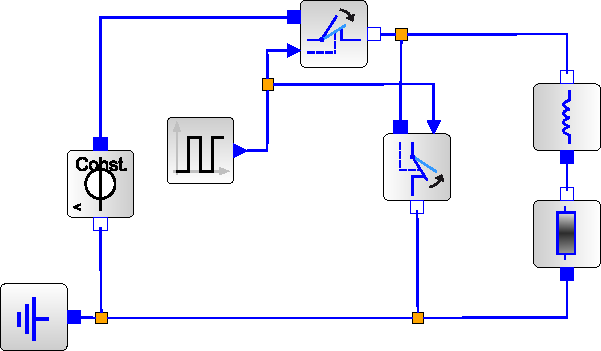
\includegraphics[width=0.4\linewidth]{img/Simu_s01}
 
\begin{minipage}{0.49\linewidth}
 \centering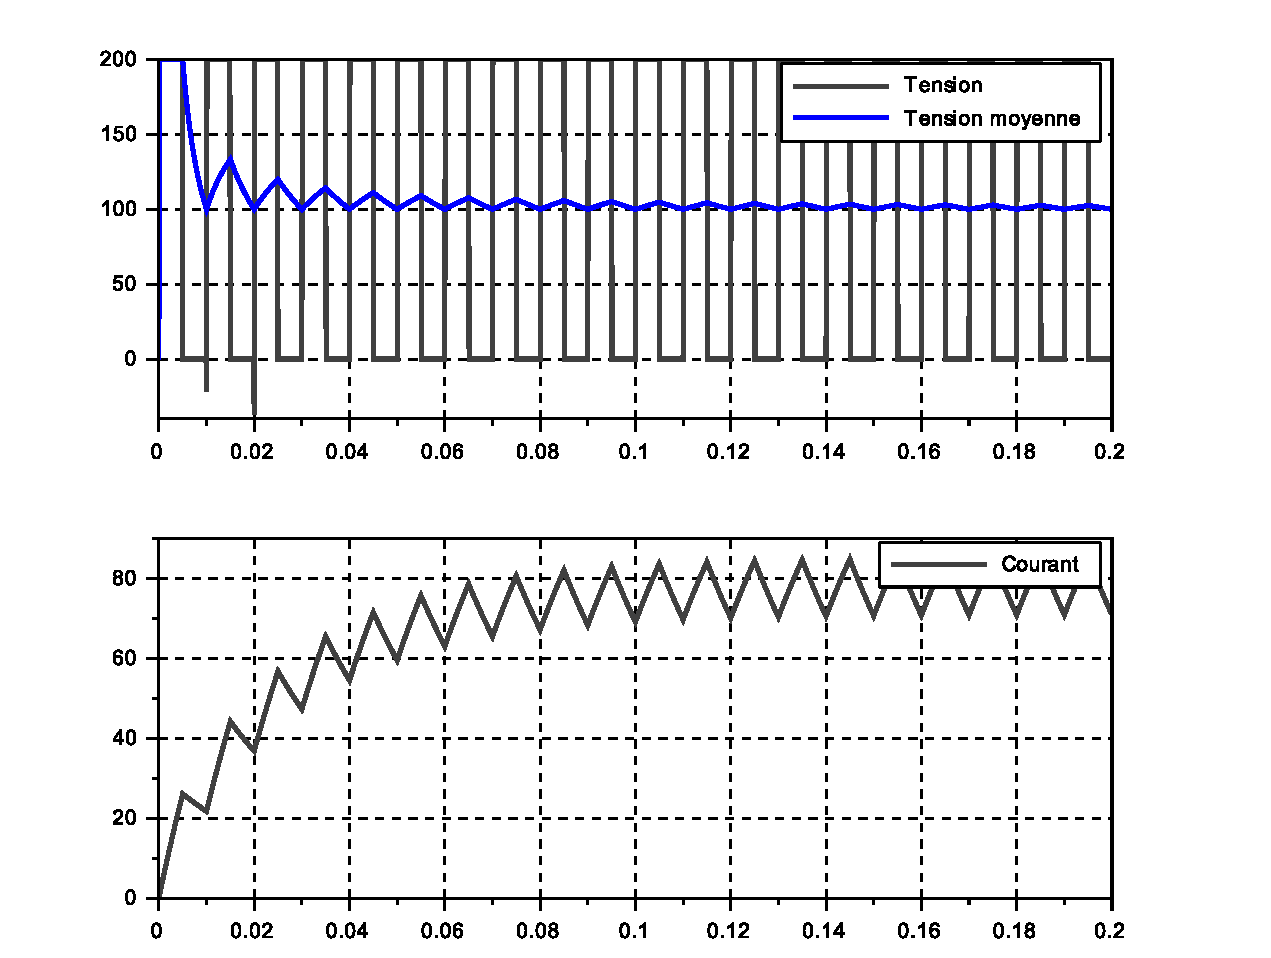
\includegraphics[width=0.9\linewidth]{img/Simu01} \\
 Fréquence de commutation de 100Hz
\end{minipage}\hfill
\begin{minipage}{0.49\linewidth}
 \centering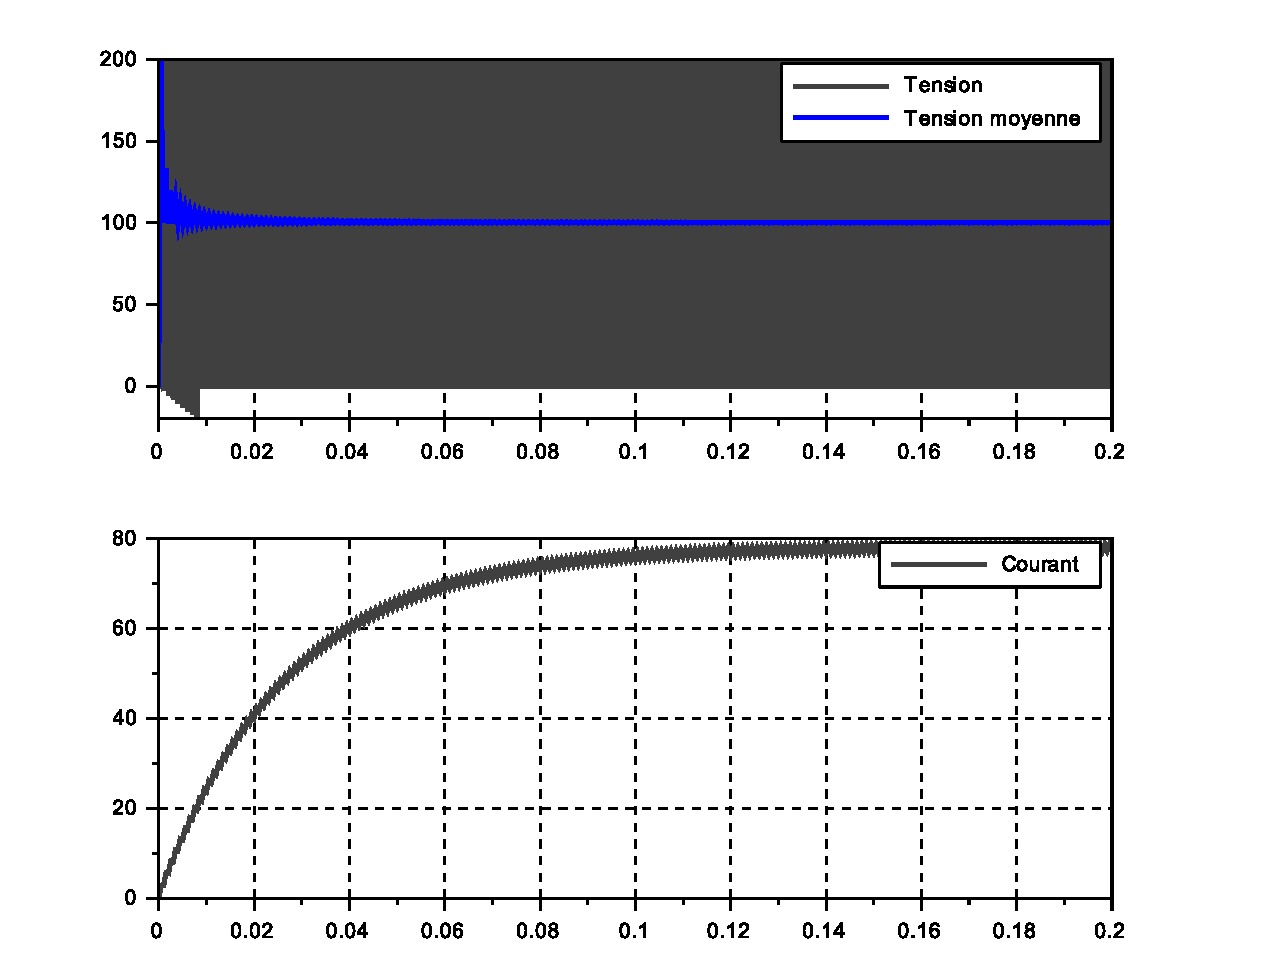
\includegraphics[width=0.9\linewidth]{img/Simu02} \\
 Fréquence de commutation de 1000Hz
\end{minipage}
}}

{\frame{
\frametitle{Source de courant R,L}

\begin{minipage}{.65\linewidth}
Il est possible alors de faire varier le \textbf{rapport cyclique} afin de \og laisser passer\fg plus ou moins d'énergie entre les deux sources.
 
Le pourcentage indique le rapport $K=\dfrac{T_h}{T}$ et le résultat est alors $U_{out}=U_L+U_R=K.U_{in}=K$.
\end{minipage}\hfill
\begin{minipage}{.3\linewidth}
\centering\begin{tikzpicture}
\draw[->] (0,0) -- (2,0);
\draw (2,0) node[below] {$t$};
\draw [->] (0,0) -- (0,1.8);
\draw[color=forestgreen,-, line width=1pt] (0,1.2) -- (1.2,1.2) -- (1.2,0) -- (1.8,0);
\draw[color=forestgreen,-, line width=1pt, dashed] (1.8,0) -- (1.8,1.2) -- (2,1.2);
\draw[triangle 45-triangle 45] (0,0.5) -- (1.2,0.5);
\draw (0.6,0.5) node[above] {$T_h$};
\draw[triangle 45-triangle 45] (0,1.5) -- (1.8,1.5);
\draw (1,1.5) node[above] {$T$};
\end{tikzpicture}
\end{minipage}
 
\begin{minipage}{0.45\linewidth}
 \centering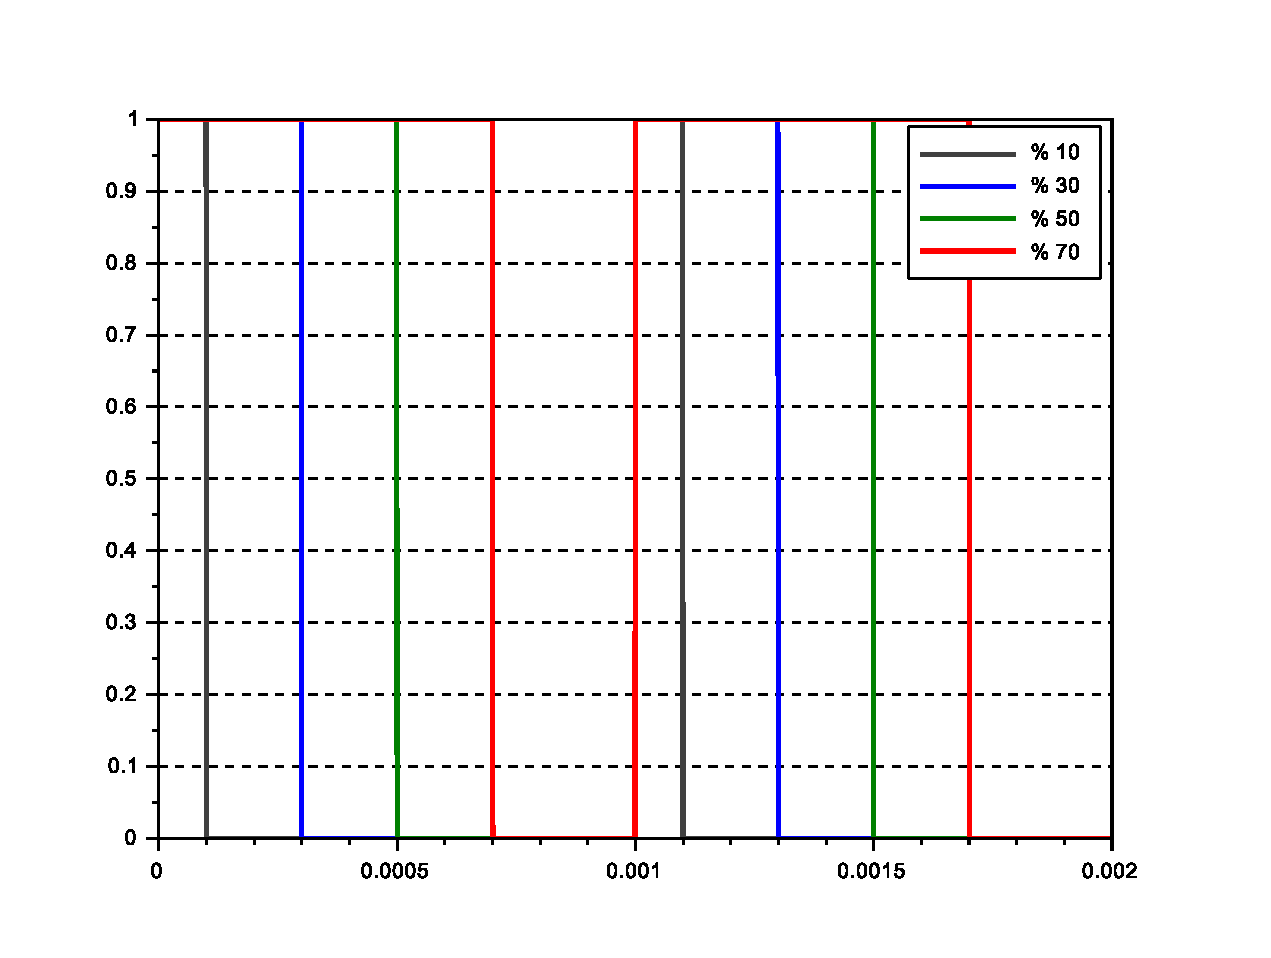
\includegraphics[width=0.9\linewidth]{img/Simu015} \\
Commande
\end{minipage}\hfill
\begin{minipage}{0.45\linewidth}
 \centering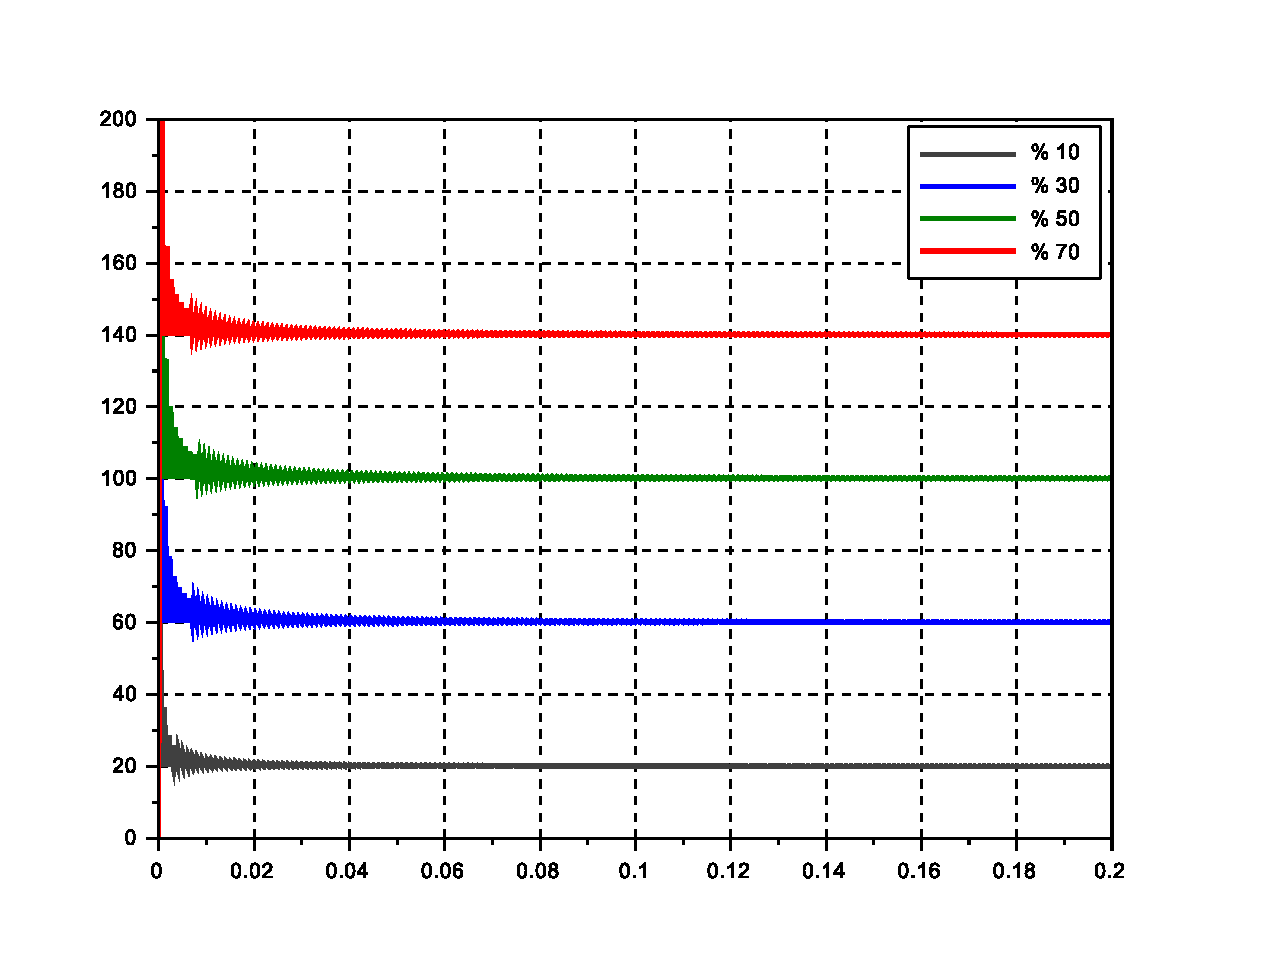
\includegraphics[width=0.9\linewidth]{img/Simu025} \\
Tension moyenne
\end{minipage}
}}

{\frame{
\frametitle{Source de courant R,L}

La simulation précédente montre l'intérêt d'un tel système. Il permet de faire varier la puissance transmise à un système électrique en jouant sur la forme d'un signal de commande.

L'analyse de la source de courant permet de faire les constats suivants :
\begin{itemize}
 \item la tension a la forme d'un créneau, ce qui peut être problématique, cependant la tension moyenne dépend de la largeur du créneau d'entrée,
 \item le courant est lissé par la bobine ($U_L=L.\dfrac{di(t)}{dt}$) et ce lissage est amélioré en augmentant la fréquence de commutation.
\end{itemize}

\begin{rem}
Le format de cette alimentation est-il compatible avec un système réel ? Par exemple, est-il possible d'alimenter un moteur électrique à l'aide d'une cellule de commutation comme celle-ci ?
\end{rem}

}}

{\frame{
\frametitle{Application: Alimentation d'un MCC}

\textit{Application:} \textbf{Distribuer} l'énergie électrique à un Moteur à Courant Continu à l'aide d'une cellule de commutation.

~\

Dans ce cas, le modèle électrique du moteur est la \textbf{source de courant}. Elle est composée d'une \textbf{inductance}, d'une \textbf{résistance} et d'une force électro-motrice (f.e.m).

~\

\begin{minipage}{0.55\linewidth}
Données de simulation:\begin{itemize}
 \item Inductance $L=12.8mH$,
 \item Résistance $R=2.84\Omega$,
 \item Alimentation $U_{in}=200V$ à $50\%$,
 \item Inertie $J_{eq}=2,05.10^{-3}kg.m^2$,
 \item Frottements secs $f=0.05N.m$,
 \item Frottements visqueux $\lambda=0.01N.m.rad^{-1}.s$.
\end{itemize}

\end{minipage}\hfill
\begin{minipage}{0.4\linewidth}
\centering\begin{circuitikz}[scale=0.8, american inductor]
\ctikzset{bipoles/length=0.8cm}
\ctikzset{inductor=american}
\draw[color=bleuf] (0,0) to[I, i<=$i$] (0,4) ;
\draw[color=bleuf] (3,0) to[V, l_=$f.e.m$] (3,1.3) to[R, l_=$R$] (3,2.6) to[L, l_=$L$, i<=$i$] (3,4) ;
\draw[color=bleuf,triangle 45-] (2.6,1.1) -- (2.6,0.2) node[left, midway] {$U_{e}$};
\draw[color=bleuf,triangle 45-] (2.6,2.4) -- (2.6,1.5) node[left, midway] {$U_{R}$};
\draw[color=bleuf,triangle 45-] (2.6,3.8) -- (2.6,2.8) node[left, midway] {$U_{L}$};
\draw[color=bleuf,triangle 45-, line width=1.5pt] (2.,2)-- (0.5,2);
\end{circuitikz}
\end{minipage}
}}

{\frame{
\frametitle{Application: Alimentation d'un MCC}

 \centering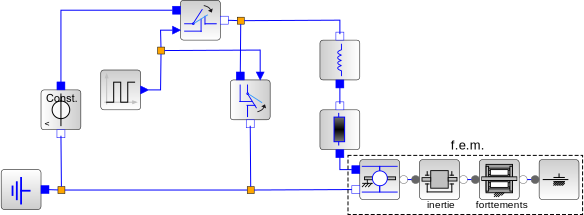
\includegraphics[width=0.6\linewidth]{img/Simu_s025}
 
\begin{minipage}{0.49\linewidth}
 \centering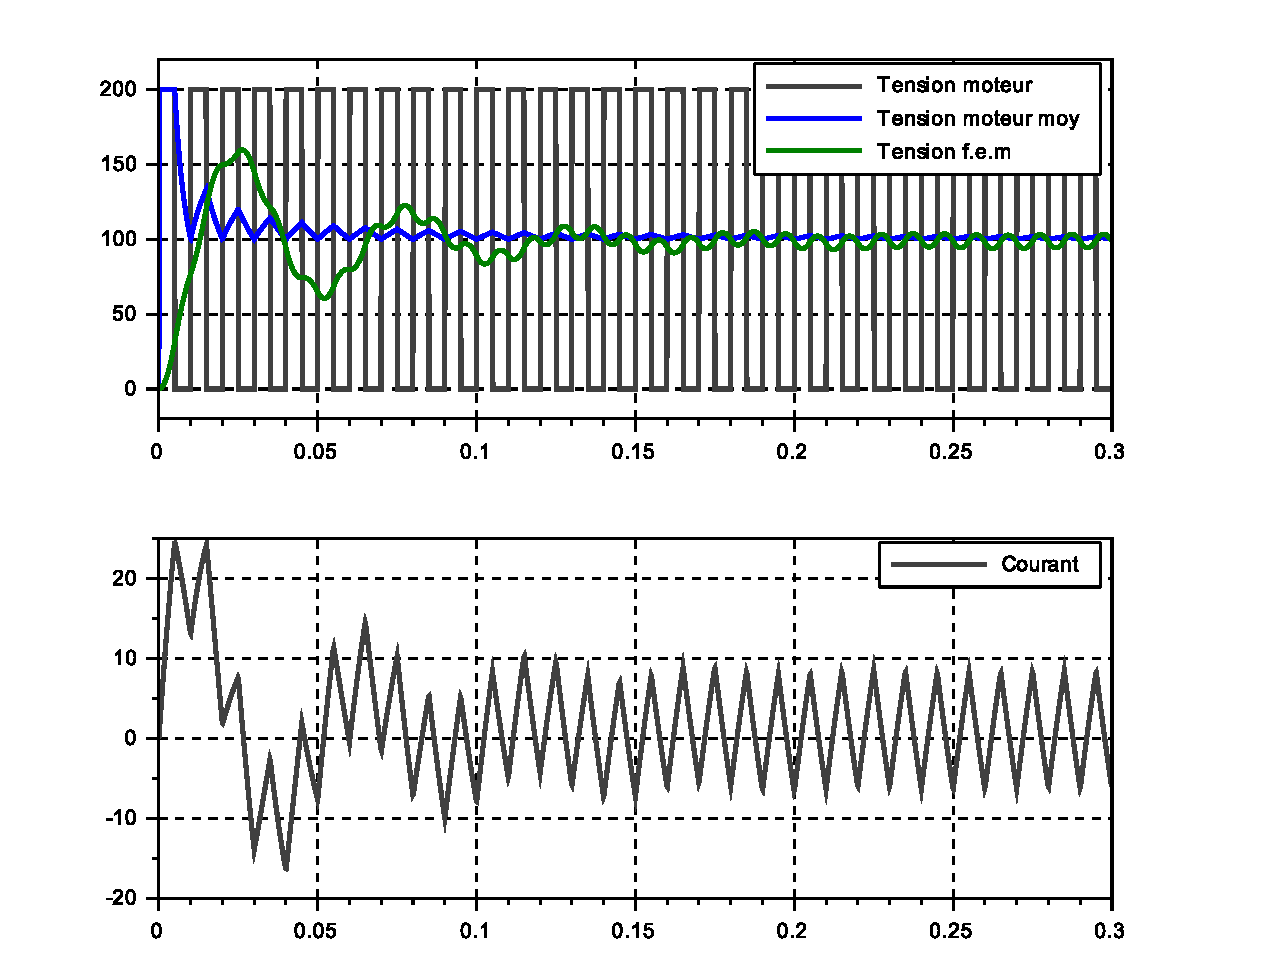
\includegraphics[width=0.9\linewidth]{img/Simu03} \\
 Fréquence de commutation de 100Hz
\end{minipage}\hfill
\begin{minipage}{0.49\linewidth}
 \centering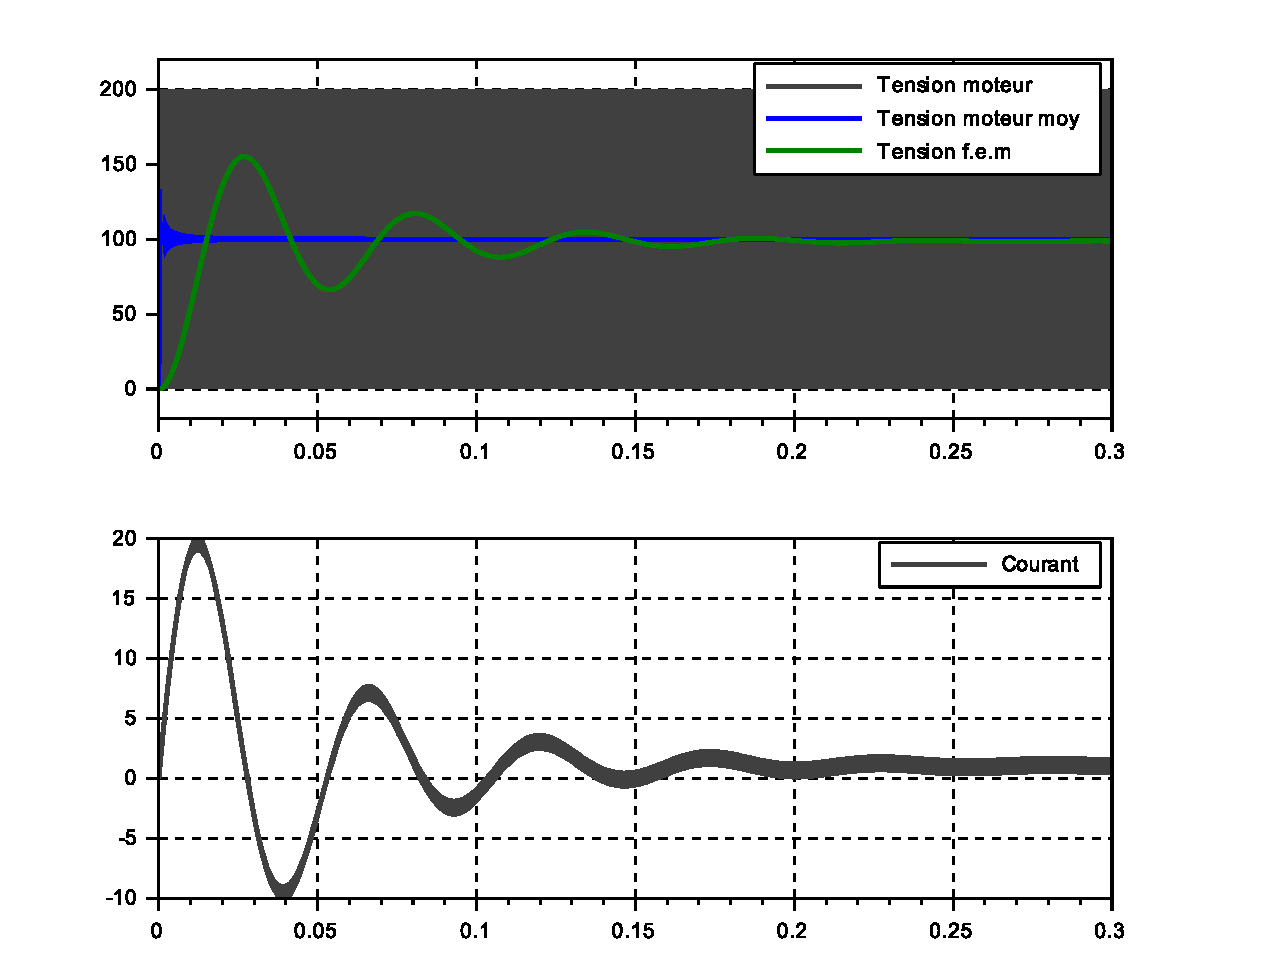
\includegraphics[width=0.9\linewidth]{img/Simu04} \\
 Fréquence de commutation de 10kHz
\end{minipage}
}}

{\frame{
\frametitle{Application: L'alimentation du MCC}

La simulation précédente montre que la forme \og créneau \fg de la tension aux bornes du moteur \textbf{ne se retrouve pas} aux bornes de la f.e.m. Cela s'explique par la loi électrique $U_e(t)=K_e.\omega(t)$. En effet, l'inertie mécanique équivalente ramenée à l'arbre du moteur empêche la variation brutale de la vitesse $\omega(t)$ et donc de la tension $U_e(t)$.

\begin{minipage}{0.45\linewidth}
Il est alors possible de choisir la tension aux bornes de la f.e.m. du moteur en fonction du rapport cyclique de la commande.

Les pics du démarrage ne reflètent pas la réalité car le modèle de simulation n'est pas valable durant cette période.
\end{minipage}\hfill
\begin{minipage}{0.45\linewidth}
\centering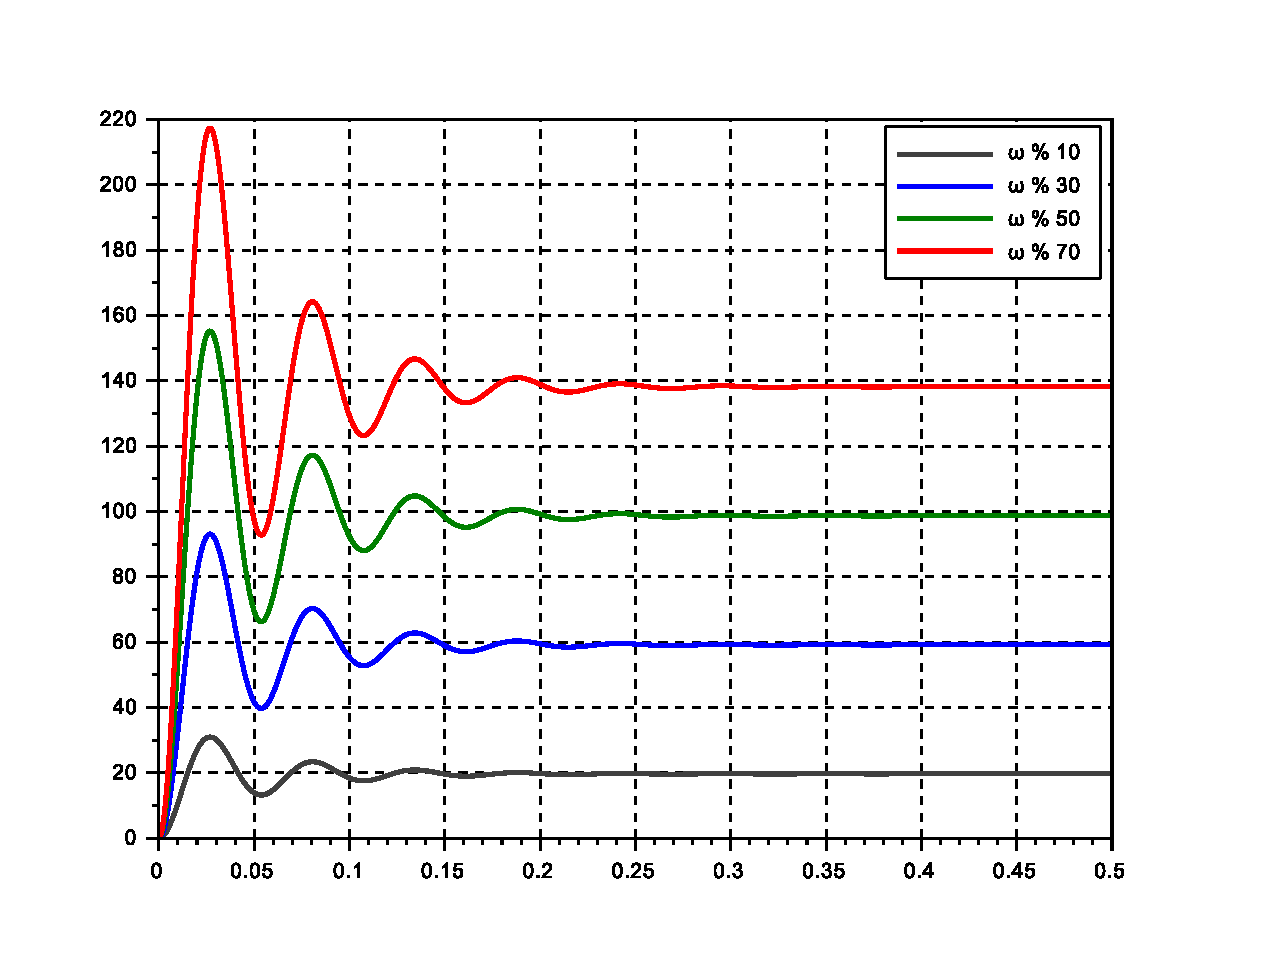
\includegraphics[width=0.9\linewidth]{img/Simu05}
\end{minipage}

\begin{resultat}
La charge peut alors être alimentée à une tension $U$ par cette \og cellule de commutation \fg avec $0<U<U_{in}$.
\end{resultat}
}}

\section{Hacheurs}

{\frame{
\frametitle{Hacheur série}

\begin{wrapfigure}[5]{r}{4cm}
\vspace{-7mm}
\centering 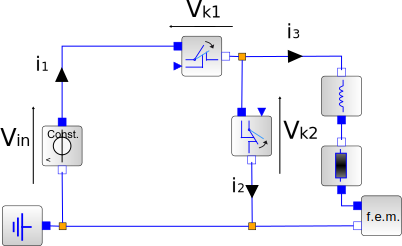
\includegraphics[width=\linewidth]{img/Simu_s0252}
\end{wrapfigure}
Afin de mettre en \oe ubre la solution retenue, il est nécessaire de déterminer quels composants permettent de jouer le rôle de ces interrupteurs.

\begin{itemize}
 \item $V_{in}=U_{k1}+U_{k2}$,
 \item $i_1=i_2+i_3$. (avec $i_3>0$, le moteur ne fonctionne pas en alternateur).
\end{itemize}

\begin{minipage}{0.24\linewidth}
\centering\begin{tikzpicture}[scale=0.6]
\draw[->] (-0.1,0) -- (3.5,0);
\draw (3.5,0) node[above] {$t$};
\draw [->] (0,-0.1) -- (0,2);
\draw (0,2) node[right] {$i_1,\textcolor{rougef}{V_{k1}}$};
\draw[-, line width=1pt] (0,0) -- (0,1) -- (0.7,1) -- (0.7,0) -- (2,0) -- (2,1) -- (2.7,1) -- (2.7,0);
\draw[-, rougef, line width=1pt, dashed] (0,0) -- (0.7,0) -- (0.7,1.2) -- (2,1.2) -- (2,0) -- (2.7,0) -- (2.7,1.2);
\draw (0.3,-0.5) node[above] {$k1$};
\draw (1.3,-0.5) node[above] {$k2$};
\draw (2.3,-0.5) node[above] {$k1$};
\end{tikzpicture}
\end{minipage}\hfill
\begin{minipage}{0.24\linewidth}
\centering\begin{tikzpicture}[scale=0.7]
\draw[->] (-1.2,0) -- (1.2,0);
\draw (1.3,0) node[above] {$V_{k1}$};
\draw [->] (0,-0.5) -- (0,1.2);
\draw (0,1.2) node[right] {$i_1$};
\draw[-] (0,1) -- (1,1);
\draw[-] (0,0.9) -- (0.9,0.9);
\draw[->] (1,0) -- (1,0.6);
\draw[-] (1,0.6) -- (1,1);
\draw[->] (0.9,0.9) -- (0.9,0.4);
\draw[-] (0.9,0.4) -- (0.9,0);
%\draw (-1,-0.5) node[] {Commandée};
\end{tikzpicture}
\end{minipage}\hfill
\begin{minipage}{0.24\linewidth}
\centering\begin{tikzpicture}[scale=0.6]
\draw[->] (-0.1,0) -- (3.5,0);
\draw (3.5,0) node[above] {$t$};
\draw [->] (0,-1) -- (0,2);
\draw (0,2) node[right] {$i_2,\textcolor{rougef}{V_{k2}}$};
\draw[-, line width=1pt] (0,0) -- (0.7,0) -- (0.7,-1) -- (2,-1) -- (2,0) -- (2.7,0) -- (2.7,-1);
\draw[-, rougef, line width=1pt, dashed] (0,0) -- (0,1.2) -- (0.7,1.2) -- (0.7,0) -- (2,0) -- (2,1.2) -- (2.7,1.2) -- (2.7,0);
\draw (0.3,-0.5) node[above] {$k1$};
\draw (1.3,-0.5) node[above] {$k2$};
\draw (2.3,-0.5) node[above] {$k1$};
\end{tikzpicture}
\end{minipage}\hfill
\begin{minipage}{0.24\linewidth}
\centering\begin{tikzpicture}[scale=0.7]
\draw[->] (-1.2,0) -- (1.2,0);
\draw (1.2,0) node[above] {$V_{k2}$};
\draw [->] (0,-1.2) -- (0,0.5);
\draw (0,0.5) node[right] {$i_2$};
\draw[-] (1,0) -- (1,-0.1);
\draw[-] (0.1,-0.1) -- (1,-0.1);
\draw[-] (0.1,-0.1) -- (0.1,-0.6);
\draw[->] (0.1,-1) -- (0.1,-0.6);
\draw[-] (0,-1) -- (0.1,-1);
\draw[->] (0,0) -- (0,-0.4);
%\draw (-1,-1.2) node[] {Spontanée};
\end{tikzpicture}
\end{minipage}

~\

Le comportement des interrupteur permet de choisir:
\begin{itemize}
 \item un IGBT pour l'interrupteur $k1$,
 \item une diode pour l'interrupteur $k2$.
\end{itemize}

}}

{\frame{
\frametitle{Hacheur série}

\begin{wrapfigure}[2]{r}{5cm}
\vspace{-20mm}
\centering \begin{tikzpicture}
\fill [bleuc] (0,0) rectangle (1,1);
\fill [bleuf] (0,0) rectangle (1,-1);
\fill [bleuf] (0,0) rectangle (-1,1);
\fill [bleuf] (0,0) rectangle (-1,-1);
\draw[->] (-1.2,0) -- (1.2,0);
\draw (1.2,-0.4) node[above] {$\omega_m$};
\draw [->] (0,-1.2) -- (0,1.2);
\draw (0,1.2) node[right] {$C_m$};
\draw (0.5,-0.5) node[] {$G$};
\draw (-0.5,0.5) node[] {$G$};
\draw (0.5,0.5) node[] {$M$};
\draw (-0.5,-0.5) node[] {$M$};
\draw (0.2,-0.2) node[] {$4$};
\draw (-0.2,0.2) node[] {$2$};
\draw (0.2,0.2) node[] {$1$};
\draw (-0.2,-0.2) node[] {$3$};
\end{tikzpicture}
\end{wrapfigure}
La solution de montage de la cellule correspondant au besoin est donc la suivante.

\bigskip

\centering\begin{circuitikz}[scale=0.8]
\ctikzset{bipoles/length=1cm}
\ctikzset{inductor=american}
\draw[color=bleuf] (4,3) node[nigbt, xscale=-1] (npn) {}
 (npn.base) node[anchor=east] {}
 (npn.collector) node[anchor=south] {}
 (npn.emitter) node[anchor=north] {};
\draw[color=bleuf] (8,0) -- (0,0) to[V, v=$U_{in}$, i>=$i_1$] (0,4) -- (4,4) -- (npn.collector);
\draw[color=bleuf] (4,0) to[Do, i<=$i_2$] (4,2) -- (npn.emitter);
\draw[color=bleuf] (4,2) to[L, l_=$L$, i>=$i_3$] (6,2) to[R, l_=$R$] (8,2) to[V, l_=$f.e.m$] (8,0) ;
\draw[color=bleuf] (3.3,2.7) edge[-triangle 45] (3.3,3.5);	
\draw[color=bleuf] node at (2.8,3) {$V_{K1}$} ;
\draw[color=bleuf] (3.3,0.7) edge[-triangle 45] (3.3,1.5);	
\draw[color=bleuf] node at (2.8,1) {$V_{K2}$} ;
\draw[color=bleuf] node at (5,3) [right]{Commande de l'IGBT} ;
\end{circuitikz}

\bigskip

Commande \textbf{sans} réversibilité de la source de courant.
}}


{\frame{
\frametitle{Hacheur 2 quadrants, réversible en courant}

\begin{wrapfigure}[4]{r}{5cm}
\vspace{-10mm}
\centering \begin{tikzpicture}
\fill [bleuc] (0,0) rectangle (1,1);
\fill [bleuc] (0,0) rectangle (1,-1);
\fill [bleuf] (0,0) rectangle (-1,1);
\fill [bleuf] (0,0) rectangle (-1,-1);
\draw[->] (-1.2,0) -- (1.2,0);
\draw (1.2,-0.4) node[above] {$\omega_m$};
\draw [->] (0,-1.2) -- (0,1.2);
\draw (0,1.2) node[right] {$C_m$};
\draw (0.5,-0.5) node[] {$G$};
\draw (-0.5,0.5) node[] {$G$};
\draw (0.5,0.5) node[] {$M$};
\draw (-0.5,-0.5) node[] {$M$};
\draw (0.2,-0.2) node[] {$4$};
\draw (-0.2,0.2) node[] {$2$};
\draw (0.2,0.2) node[] {$1$};
\draw (-0.2,-0.2) node[] {$3$};
\end{tikzpicture}
\end{wrapfigure}
En choisissant de permettre l'utilisation du moteur en alternateur, il faut alors autoriser la réversibilité en courant. Attention dans cette solution la vitesse de rotation est toujours positive.

\begin{minipage}{0.45\linewidth}
\begin{itemize}
 \item $V_{in}=U_{k1}+U_{k2}$,
 \item $i_1=i_2+i_3$. (avec $i_3$ quelconque).
\end{itemize}
\end{minipage}\hfill
\begin{minipage}{0.45\linewidth}
Commande \textbf{avec} réversibilité de la source de courant.
\end{minipage}

\centering\begin{circuitikz}[scale=0.8]
\ctikzset{bipoles/length=0.8cm}
\ctikzset{inductor=american}
\draw[color=bleuf] (2,3) node[nigbt] (npn) {}
 (npn.base) node[anchor=east] {}
 (npn.collector) node[anchor=south] {}
 (npn.emitter) node[anchor=north] {};
 \draw[color=bleuf] (2,1) node[nigbt] (npn2) {}
 (npn2.base) node[anchor=east] {}
 (npn2.collector) node[anchor=south] {}
 (npn2.emitter) node[anchor=north] {};
\draw[color=bleuf] (8,0) -- (0,0) to[V, v=$U_{in}$] (0,4) -- (4,4) (2,4) -- (npn.collector);
\draw[color=bleuf] (4,0) to[Do] (4,2) to[Do] (4,4);
\draw[color=bleuf] (2,0) -- (npn2.emitter)  (npn2.collector)-- (npn.emitter);
\draw[color=bleuf] (2,2) -- (4,2);
\draw[color=bleuf] (4,2) to[L, l_=$L$] (6,2) to[R, l_=$R$] (8,2) to[V, l_=$f.e.m$] (8,0) ;
\end{circuitikz}
}}

{\frame{
\frametitle{Hacheur 2 quadrants, réversible en courant}

\textbf{Moteur}

\begin{minipage}{0.45\linewidth}
\centering\begin{circuitikz}[scale=0.6]
\ctikzset{bipoles/length=0.6cm}
\ctikzset{inductor=american}
\node(0) at (5,2)[color=bleuf,shape=circle,draw] {M};
\draw[color=bleuf] (2,3) node[nigbt, scale=0.5] (npn) {}
 (npn.base) node[anchor=east] {}
 (npn.collector) node[anchor=south] {}
 (npn.emitter) node[anchor=north] {};
 \draw[color=bleuf, dashed] (2,1) node[nigbt, scale=0.5] (npn2) {}
 (npn2.base) node[anchor=east] {}
 (npn2.collector) node[anchor=south] {}
 (npn2.emitter) node[anchor=north] {};
\draw[color=bleuf] (6,0) -- (0,0) to[V, v=$U_{in}$] (0,4) -- (2,4) -- (npn.collector);
\draw[color=bleuf, dashed] (4,0) to[Do] (4,2) to[Do] (4,4) -- (2,4);
\draw[color=bleuf, dashed] (2,0) -- (npn2.emitter) (npn2.collector) -- (2,2);
\draw[color=bleuf] (2,2) -- (npn.emitter);
\draw[color=bleuf] (2,2) -- (4,2);
\draw[color=bleuf] (4,2) -- (0) -- (6,2) -- (6,0) ;
\end{circuitikz}
\end{minipage}\hfill
\begin{minipage}{0.45\linewidth}
\centering\begin{circuitikz}[scale=0.6]
\ctikzset{bipoles/length=0.6cm}
\ctikzset{inductor=american}
\node(0) at (5,2)[color=bleuf,shape=circle,draw] {M};
\draw[color=bleuf, dashed] (2,3) node[nigbt, scale=0.5] (npn) {}
 (npn.base) node[anchor=east] {}
 (npn.collector) node[anchor=south] {}
 (npn.emitter) node[anchor=north] {};
 \draw[color=bleuf, dashed] (2,1) node[nigbt, scale=0.5] (npn2) {}
 (npn2.base) node[anchor=east] {}
 (npn2.collector) node[anchor=south] {}
 (npn2.emitter) node[anchor=north] {};
\draw[color=bleuf] (6,0) -- (4,0);
\draw[color=bleuf, dashed] (4,0) -- (0,0) to[V, v=$U_{in}$] (0,4) -- (4,4) (2,4) -- (npn.collector);
\draw[color=bleuf] (4,0) to[Do] (4,2);
\draw[color=bleuf, dashed] (4,2) to[Do] (4,4);
\draw[color=bleuf, dashed] (2,0) -- (npn2.emitter)  (npn2.collector)-- (npn.emitter);
\draw[color=bleuf, dashed] (2,2) -- (4,2);
\draw[color=bleuf] (4,2) -- (0) -- (6,2) -- (6,0) ;
\end{circuitikz}
\end{minipage}

\textbf{Générateur}

\begin{minipage}{0.45\linewidth}
\centering\begin{circuitikz}[scale=0.6]
\ctikzset{bipoles/length=0.6cm}
\ctikzset{inductor=american}
\node(0) at (5,2)[color=bleuf,shape=circle,draw] {M};
\draw[color=bleuf, dashed] (2,3) node[nigbt, scale=0.5] (npn) {}
 (npn.base) node[anchor=east] {}
 (npn.collector) node[anchor=south] {}
 (npn.emitter) node[anchor=north] {};
 \draw[color=bleuf, dashed] (2,1) node[nigbt, scale=0.5] (npn2) {}
 (npn2.base) node[anchor=east] {}
 (npn2.collector) node[anchor=south] {}
 (npn2.emitter) node[anchor=north] {};
\draw[color=bleuf] (6,0) -- (0,0) to[V, v=$U_{in}$] (0,4) --(2,4);
\draw[color=bleuf, dashed] (2,4) -- (npn.collector);
\draw[color=bleuf, dashed] (4,0) to[Do] (4,2);
\draw[color=bleuf] (4,2) to[Do] (4,4) -- (2,4);
\draw[color=bleuf, dashed] (2,0) -- (npn2.emitter) (npn2.collector) -- (2,2);
\draw[color=bleuf, dashed] (2,2) -- (npn.emitter);
\draw[color=bleuf, dashed] (2,2) -- (4,2);
\draw[color=bleuf] (4,2) -- (0) -- (6,2) -- (6,0) ;
\end{circuitikz}
\end{minipage}\hfill
\begin{minipage}{0.45\linewidth}
\centering\begin{circuitikz}[scale=0.6]
\ctikzset{bipoles/length=0.6cm}
\ctikzset{inductor=american}
\node(0) at (5,2)[color=bleuf,shape=circle,draw] {M};
\draw[color=bleuf, dashed] (2,3) node[nigbt, scale=0.5] (npn) {}
 (npn.base) node[anchor=east] {}
 (npn.collector) node[anchor=south] {}
 (npn.emitter) node[anchor=north] {};
 \draw[color=bleuf] (2,1) node[nigbt, scale=0.5] (npn2) {}
 (npn2.base) node[anchor=east] {}
 (npn2.collector) node[anchor=south] {}
 (npn2.emitter) node[anchor=north] {};
\draw[color=bleuf] (6,0) -- (2,0);
\draw[color=bleuf, dashed] (2,0) -- (0,0) to[V, v=$U_{in}$] (0,4) -- (4,4) (2,4) -- (npn.collector);
\draw[color=bleuf, dashed] (4,0) to[Do] (4,2) to[Do] (4,4);
\draw[color=bleuf] (2,0) -- (npn2.emitter)  (npn2.collector)-- (2,2);
\draw[color=bleuf, dashed] (2,2) -- (npn.emitter);
\draw[color=bleuf] (2,2) -- (4,2);
\draw[color=bleuf] (4,2) -- (0) -- (6,2) -- (6,0) ;
\end{circuitikz}
\end{minipage}
}}

{\frame{
\frametitle{Hacheur 4 quadrants}

\begin{wrapfigure}[5]{r}{5cm}
\vspace{-7mm}
\centering \begin{tikzpicture}
\fill [bleuc] (0,0) rectangle (1,1);
\fill [bleuc] (0,0) rectangle (1,-1);
\fill [bleuc] (0,0) rectangle (-1,1);
\fill [bleuc] (0,0) rectangle (-1,-1);
\draw[->] (-1.2,0) -- (1.2,0);
\draw (1.2,-0.4) node[above] {$\omega_m$};
\draw [->] (0,-1.2) -- (0,1.2);
\draw (0,1.2) node[right] {$C_m$};
\draw (0.5,-0.5) node[] {$G$};
\draw (-0.5,0.5) node[] {$G$};
\draw (0.5,0.5) node[] {$M$};
\draw (-0.5,-0.5) node[] {$M$};
\draw (0.2,-0.2) node[] {$4$};
\draw (-0.2,0.2) node[] {$2$};
\draw (0.2,0.2) node[] {$1$};
\draw (-0.2,-0.2) node[] {$3$};
\end{tikzpicture}
\end{wrapfigure}
Le dernier cas consiste à permettre la réversibilité en tension (choix du \textit{sens de rotation} d'un moteur). Cela revient à alimenter la charge avec une tension $U$ telle que $-U_{in}<U<U_{in}$.

La \textbf{configuration d'interrupteurs} suivante permet cette application.

\vspace{1cm}

\begin{minipage}{0.48\linewidth}
\begin{circuitikz}[scale=0.6]
\ctikzset{bipoles/length=0.8cm}
\draw[color=bleuf] (3,1) -- (0,1)  to[V=$U_{in}$] (0,4) -- (3,4) 
(3,2.5) to[I, i=$i$] (6,2.5)
node[ocirc] (A) at (3,3.5) {}
node[ocirc] (B) at (3,2) {}
node[ocirc] (C) at (6,3.5) {}
node[ocirc] (D) at (6,2) {} ;
\draw[color=bleuf, dashed] (3,1) -- (3,1.4) -- (2.7,2) (B) -- (3,2.5)
(6,2.5) -- (6,2.9) -- (5.7,3.5) (C) -- (6,4)
(3,4) -- (6,4);
\draw[color=bleuf] (3,2.5) -- (3,2.9) -- (2.9,3.5) (A) -- (3,4)
(6,1) -- (6,1.4) -- (5.9,2) (D) -- (6,2.5)
(6,1) -- (3,1);
\draw (5,1.8) edge[-stealth] (4,1.8);
\node (U) at (4.5,1.5){$u$};
\draw[color=bleuf] node at (3.4,3.3) {$K_1$} ;
\draw[color=bleuf] node at (3.4,1.8) {$K_2$} ;
\draw[color=bleuf] node at (6.4,3.3) {$K_3$} ;
\draw[color=bleuf] node at (6.4,1.8) {$K_4$} ;
\end{circuitikz}
\end{minipage}\hfill
\begin{minipage}{0.48\linewidth}
\begin{circuitikz}[scale=0.6]
\ctikzset{bipoles/length=0.8cm}
\draw[color=bleuf] (3,1) -- (0,1)  to[V=$U_{in}$] (0,4) -- (3,4) 
(3,2.5) to[I, i<=$i$] (6,2.5)
node[ocirc] (A) at (3,3.5) {}
node[ocirc] (B) at (3,2) {}
node[ocirc] (C) at (6,3.5) {}
node[ocirc] (D) at (6,2) {} ;
\draw[color=bleuf] (3,1) -- (3,1.4) -- (2.9,2) (B) -- (3,2.5)
(6,2.5) -- (6,2.9) -- (5.9,3.5) (C) -- (6,4)
(3,4) -- (6,4);
\draw[color=bleuf, dashed] (3,2.5) -- (3,2.9) -- (2.7,3.5) (A) -- (3,4)
(6,1) -- (6,1.4) -- (5.7,2) (D) -- (6,2.5)
(6,1) -- (3,1);
\draw (4,1.8) edge[-stealth] (5,1.8);
\node (U) at (4.5,1.5){$u$};
\draw[color=bleuf] node at (3.4,3.3) {$K_1$} ;
\draw[color=bleuf] node at (3.4,1.8) {$K_2$} ;
\draw[color=bleuf] node at (6.4,3.3) {$K_3$} ;
\draw[color=bleuf] node at (6.4,1.8) {$K_4$} ;
\end{circuitikz}
\end{minipage}
}}

{\frame{
\frametitle{Hacheur 4 quadrants}

\begin{minipage}{0.55\linewidth}
 \centering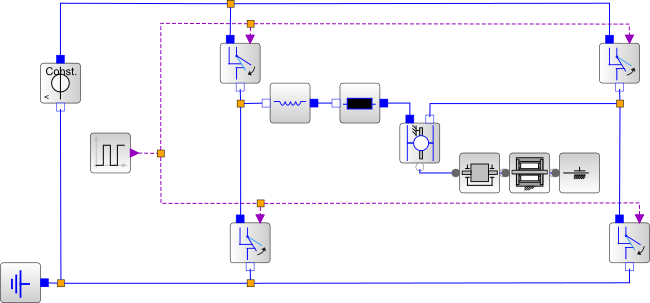
\includegraphics[width=0.9\linewidth]{img/Simu_s03}
\end{minipage}\hfill
\begin{minipage}{0.38\linewidth}
Cette configuration a été mise en place sur le modèle de simulation précédent.

Il est alors possible de gérer le signe de la tension aux bornes de la f.e.m.
\end{minipage}

La tension $U_{out}$ est donc la moyenne entre $U_{in}$ et $-U_{in}$ pondérée du rapport cyclique.

\begin{minipage}{0.48\linewidth}
\fbox{$U_{out}=U_{in}.K-U_{in}.(100-K)=U_{in}.(2.K-100)$}

Ainsi:
\begin{itemize}
 \item $K=50\%$: $U_{fem}=0$,
 \item $K>50\%$: $U_{fem}>0$,
 \item $K<50\%$: $U_{fem}<0$,
\end{itemize}

\end{minipage}\hfill
\begin{minipage}{0.48\linewidth}
 \centering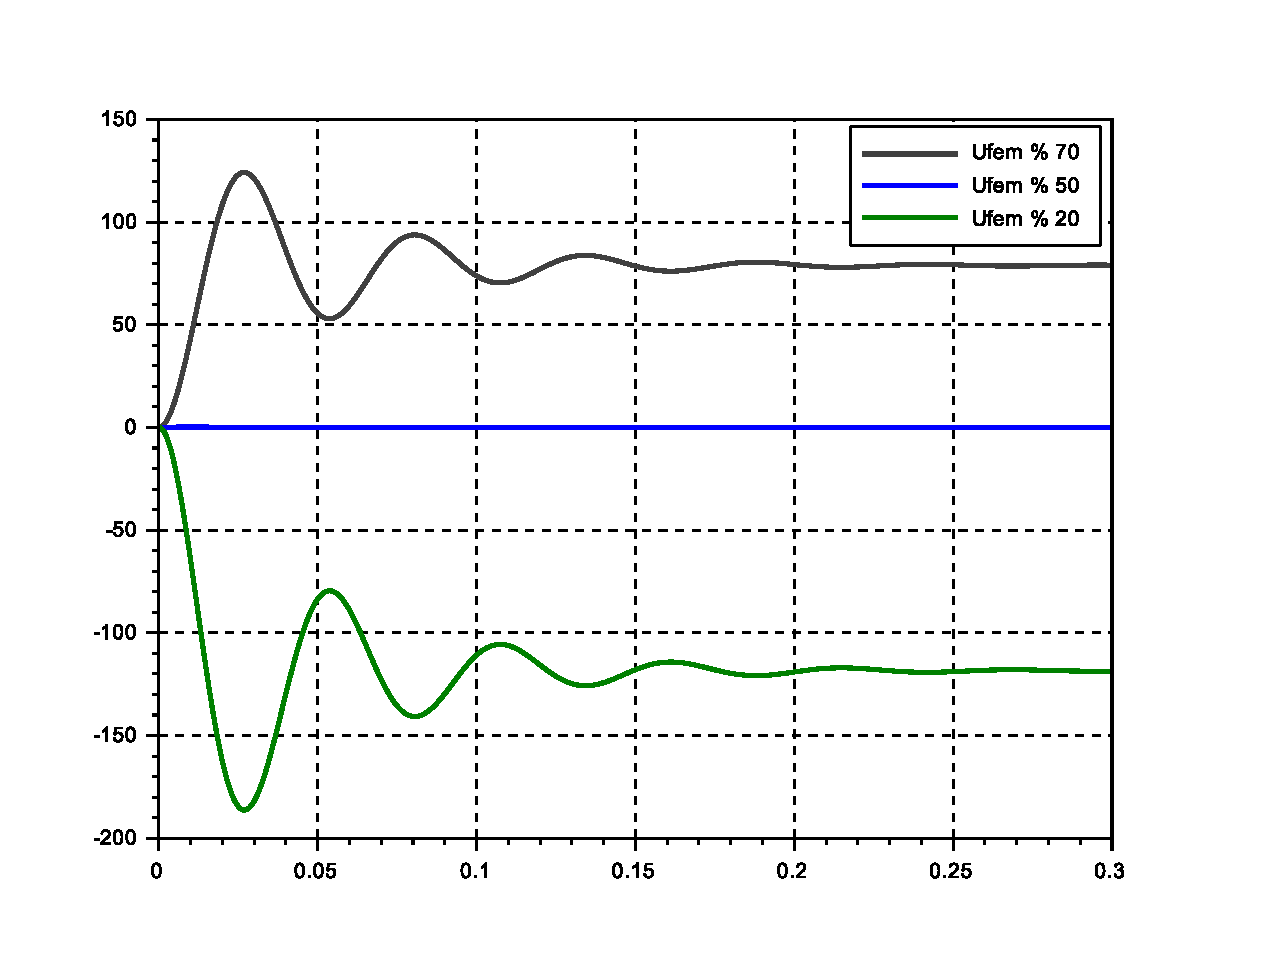
\includegraphics[width=0.9\linewidth]{img/Simu06}
\end{minipage}
}}

{\frame{
\frametitle{Hacheur 4 quadrants}

\begin{center}
\begin{circuitikz}[scale=0.8]
\ctikzset{bipoles/length=0.8cm}
\node(0) at (4.5,2)[color=bleuf,shape=circle,draw] {M};
\draw[color=bleuf] (2,3) node[nigbt] (npn) {}
 (npn.base) node[anchor=east] {}
 (npn.collector) node[anchor=south] {}
 (npn.emitter) node[anchor=north] {};
 \draw[color=bleuf] (2,1) node[nigbt] (npn2) {}
 (npn2.base) node[anchor=east] {}
 (npn2.collector) node[anchor=south] {}
 (npn2.emitter) node[anchor=north] {};
 \draw[color=bleuf] (6,3) node[nigbt] (npn3) {}
 (npn3.base) node[anchor=east] {}
 (npn3.collector) node[anchor=south] {}
 (npn3.emitter) node[anchor=north] {};
 \draw[color=bleuf] (6,1) node[nigbt] (npn4) {}
 (npn4.base) node[anchor=east] {}
 (npn4.collector) node[anchor=south] {}
 (npn4.emitter) node[anchor=north] {};
 \draw[color=bleuf] (7,0) -- (0,0)  to[V=$U_{in}$] (0,4) -- (7,4);
 \draw[color=bleuf] (2,0) --  (npn2.emitter)  (npn2.collector) -- (npn.emitter) (npn.collector) -- (2,4);
 \draw[color=bleuf] (6,0) --  (npn4.emitter)  (npn4.collector) -- (npn3.emitter) (npn3.collector) -- (6,4);
 \draw[color=bleuf] (3,0) to[Do] (3,2) to[Do] (3,4) ;
 \draw[color=bleuf] (7,0) to[Do] (7,2) to[Do] (7,4) ;
 \draw[color=bleuf] (2,2) -- (0) -- (7,2) ;
 \node (K1) at (2.4,3){$K_1$};
 \node (K1) at (2.4,1){$K_2$};
 \node (K1) at (6.4,3){$K_3$};
 \node (K1) at (6.4,1){$K_4$};
\end{circuitikz}
\end{center}

La commutation combinée des IGBT $K_1$, $K_2$, $K_3$ et $K_4$ va permettre les comportements des 4 quadrants suivants:
\begin{itemize}
 \item Quadrant 1: MCC fonctionne en moteur tournant dans le sens positif,
 \item Quadrant 2: MCC fonctionne en générateur tournant dans le sens négatif,
 \item Quadrant 3: MCC fonctionne en moteur tournant dans le sens négatif,
 \item Quadrant 4: MCC fonctionne en générateur tournant dans le sens positif.
\end{itemize}

}}

{\frame{
\frametitle{Quadrant 1: Moteur, sens positif}

\begin{minipage}{0.45\linewidth}
\centering\begin{circuitikz}[scale=0.6]
\ctikzset{bipoles/length=0.6cm}
\node(0) at (4.5,2)[color=bleuf,shape=circle,draw] {M};
\draw[color=bleuf] (2,3) node[nigbt, scale=0.5] (npn) {}
 (npn.base) node[anchor=east] {}
 (npn.collector) node[anchor=south] {}
 (npn.emitter) node[anchor=north] {};
 \draw[color=bleuf, dashed] (2,1) node[nigbt, scale=0.5] (npn2) {}
 (npn2.base) node[anchor=east] {}
 (npn2.collector) node[anchor=south] {}
 (npn2.emitter) node[anchor=north] {};
 \draw[color=bleuf, dashed] (6,3) node[nigbt, scale=0.5] (npn3) {}
 (npn3.base) node[anchor=east] {}
 (npn3.collector) node[anchor=south] {}
 (npn3.emitter) node[anchor=north] {};
 \draw[color=bleuf] (6,1) node[nigbt, scale=0.5] (npn4) {}
 (npn4.base) node[anchor=east] {}
 (npn4.collector) node[anchor=south] {}
 (npn4.emitter) node[anchor=north] {};
 \draw[color=bleuf, dashed] (7,0) -- (6,0);
 \draw[color=bleuf] (6,0) -- (0,0)  to[V=$U_{in}$] (0,4) -- (2,4);
 \draw[color=bleuf, dashed] (2,4) -- (7,4) ;
 \draw[color=bleuf, dashed] (2,0) -- (npn2.emitter)  (npn2.collector) -- (2,2);
 \draw[color=bleuf] (2,2) -- (npn.emitter) (npn.collector) -- (2,4);
 \draw[color=bleuf] (6,0) -- (npn4.emitter)  (npn4.collector) -- (6,2) ;
 \draw[color=bleuf, dashed] (6,2) -- (npn3.emitter) (npn3.collector) -- (6,4);
 \draw[color=bleuf, dashed] (3,0) to[Do] (3,2) ;
 \draw[color=bleuf, dashed] (3,2) to[Do] (3,4) ;
 \draw[color=bleuf, dashed] (7,0) to[Do] (7,2) ;
 \draw[color=bleuf, dashed] (7,2) to[Do] (7,4) ;
 \draw[color=bleuf] (2,2) -- (0) -- (6,2) ;
 \draw[color=bleuf, dashed] (6,2) -- (7,2) ;
 \node (K) at (4,-0.5){$K_1$ et $K_4$};
\end{circuitikz}
\end{minipage}\hfill
\begin{minipage}{0.45\linewidth}
\centering\begin{circuitikz}[scale=0.6]
\ctikzset{bipoles/length=0.6cm}
\node(0) at (4.5,2)[color=bleuf,shape=circle,draw] {M};
\draw[color=bleuf] (2,3) node[nigbt, scale=0.5] (npn) {}
 (npn.base) node[anchor=east] {}
 (npn.collector) node[anchor=south] {}
 (npn.emitter) node[anchor=north] {};
 \draw[color=bleuf, dashed] (2,1) node[nigbt, scale=0.5] (npn2) {}
 (npn2.base) node[anchor=east] {}
 (npn2.collector) node[anchor=south] {}
 (npn2.emitter) node[anchor=north] {};
 \draw[color=bleuf, dashed] (6,3) node[nigbt, scale=0.5] (npn3) {}
 (npn3.base) node[anchor=east] {}
 (npn3.collector) node[anchor=south] {}
 (npn3.emitter) node[anchor=north] {};
 \draw[color=bleuf, dashed] (6,1) node[nigbt, scale=0.5] (npn4) {}
 (npn4.base) node[anchor=east] {}
 (npn4.collector) node[anchor=south] {}
 (npn4.emitter) node[anchor=north] {};
 \draw[color=bleuf, dashed] (7,0) -- (0,0)  to[V=$U_{in}$] (0,4) -- (2,4);
 \draw[color=bleuf] (2,4) -- (7,4) ;
 \draw[color=bleuf, dashed] (2,0) -- (npn2.emitter)  (npn2.collector) -- (2,2);
 \draw[color=bleuf] (2,2) -- (npn.emitter) (npn.collector) -- (2,4);
 \draw[color=bleuf, dashed] (6,0) -- (npn4.emitter)  (npn4.collector) -- (6,2) ;
 \draw[color=bleuf, dashed] (6,2) -- (npn3.emitter) (npn3.collector) -- (6,4);
 \draw[color=bleuf, dashed] (3,0) to[Do] (3,2) ;
 \draw[color=bleuf, dashed] (3,2) to[Do] (3,4) ;
 \draw[color=bleuf, dashed] (7,0) to[Do] (7,2) ;
 \draw[color=bleuf] (7,2) to[Do] (7,4) ;
 \draw[color=bleuf] (2,2) -- (0) -- (7,2) ;
  \node (K) at (4,-0.5){$K_1$ et $D_3$};
\end{circuitikz}
\end{minipage}

\bigskip

\begin{minipage}{0.45\linewidth}
\centering\begin{circuitikz}[scale=0.6]
\ctikzset{bipoles/length=0.6cm}
\node(0) at (4.5,2)[color=bleuf,shape=circle,draw] {M};
\draw[color=bleuf] (2,3) node[nigbt, scale=0.5] (npn) {}
 (npn.base) node[anchor=east] {}
 (npn.collector) node[anchor=south] {}
 (npn.emitter) node[anchor=north] {};
 \draw[color=bleuf, dashed] (2,1) node[nigbt, scale=0.5] (npn2) {}
 (npn2.base) node[anchor=east] {}
 (npn2.collector) node[anchor=south] {}
 (npn2.emitter) node[anchor=north] {};
 \draw[color=bleuf, dashed] (6,3) node[nigbt, scale=0.5] (npn3) {}
 (npn3.base) node[anchor=east] {}
 (npn3.collector) node[anchor=south] {}
 (npn3.emitter) node[anchor=north] {};
 \draw[color=bleuf] (6,1) node[nigbt, scale=0.5] (npn4) {}
 (npn4.base) node[anchor=east] {}
 (npn4.collector) node[anchor=south] {}
 (npn4.emitter) node[anchor=north] {};
 \draw[color=bleuf, dashed] (7,0) -- (6,0);
 \draw[color=bleuf] (6,0) -- (0,0)  to[V=$U_{in}$] (0,4) -- (2,4);
 \draw[color=bleuf, dashed] (2,4) -- (7,4) ;
 \draw[color=bleuf, dashed] (2,0) -- (npn2.emitter)  (npn2.collector) -- (2,2);
 \draw[color=bleuf] (2,2) -- (npn.emitter) (npn.collector) -- (2,4);
 \draw[color=bleuf] (6,0) -- (npn4.emitter)  (npn4.collector) -- (6,2) ;
 \draw[color=bleuf, dashed] (6,2) -- (npn3.emitter) (npn3.collector) -- (6,4);
 \draw[color=bleuf, dashed] (3,0) to[Do] (3,2) ;
 \draw[color=bleuf, dashed] (3,2) to[Do] (3,4) ;
 \draw[color=bleuf, dashed] (7,0) to[Do] (7,2) ;
 \draw[color=bleuf, dashed] (7,2) to[Do] (7,4) ;
 \draw[color=bleuf] (2,2) -- (0) -- (6,2) ;
 \draw[color=bleuf, dashed] (6,2) -- (7,2) ;
 \node (K) at (4,-0.5){$K_1$ et $K_4$};
\end{circuitikz}
\end{minipage}\hfill
\begin{minipage}{0.45\linewidth}
\centering\begin{circuitikz}[scale=0.6]
\ctikzset{bipoles/length=0.6cm}
\node(0) at (4.5,2)[color=bleuf,shape=circle,draw] {M};
\draw[color=bleuf, dashed] (2,3) node[nigbt, scale=0.5] (npn) {}
 (npn.base) node[anchor=east] {}
 (npn.collector) node[anchor=south] {}
 (npn.emitter) node[anchor=north] {};
 \draw[color=bleuf, dashed] (2,1) node[nigbt, scale=0.5] (npn2) {}
 (npn2.base) node[anchor=east] {}
 (npn2.collector) node[anchor=south] {}
 (npn2.emitter) node[anchor=north] {};
 \draw[color=bleuf, dashed] (6,3) node[nigbt, scale=0.5] (npn3) {}
 (npn3.base) node[anchor=east] {}
 (npn3.collector) node[anchor=south] {}
 (npn3.emitter) node[anchor=north] {};
 \draw[color=bleuf] (6,1) node[nigbt, scale=0.5] (npn4) {}
 (npn4.base) node[anchor=east] {}
 (npn4.collector) node[anchor=south] {}
 (npn4.emitter) node[anchor=north] {};
 \draw[color=bleuf, dashed] (7,0) -- (6,0) (3,0) -- (0,0)  to[V=$U_{in}$] (0,4) -- (2,4);;
 \draw[color=bleuf] (6,0) -- (3,0);
 \draw[color=bleuf, dashed] (2,4) -- (7,4) ;
 \draw[color=bleuf, dashed] (2,0) -- (npn2.emitter)  (npn2.collector) -- (2,2);
 \draw[color=bleuf, dashed] (2,2) -- (npn.emitter) (npn.collector) -- (2,4);
 \draw[color=bleuf] (6,0) -- (npn4.emitter)  (npn4.collector) -- (6,2) ;
 \draw[color=bleuf, dashed] (6,2) -- (npn3.emitter) (npn3.collector) -- (6,4);
 \draw[color=bleuf] (3,0) to[Do] (3,2) ;
 \draw[color=bleuf, dashed] (3,2) to[Do] (3,4) ;
 \draw[color=bleuf, dashed] (7,0) to[Do] (7,2) ;
 \draw[color=bleuf, dashed] (7,2) to[Do] (7,4) ;
 \draw[color=bleuf, dashed] (2,2) -- (3,2) ;
 \draw[color=bleuf] (3,2) -- (0) -- (6,2) ;
 \draw[color=bleuf, dashed] (6,2) -- (7,2) ;
 \node (K) at (4,-0.5){$K_4$ et $D_2$};
\end{circuitikz}
\end{minipage}
}}

{\frame{
\frametitle{Quadrant 2: Générateur sens négatif}

\begin{minipage}{0.45\linewidth}
\centering\begin{circuitikz}[scale=0.6]
\ctikzset{bipoles/length=0.6cm}
\node(0) at (4.5,2)[color=bleuf,shape=circle,draw] {M};
\draw[color=bleuf, dashed] (2,3) node[nigbt, scale=0.5] (npn) {}
 (npn.base) node[anchor=east] {}
 (npn.collector) node[anchor=south] {}
 (npn.emitter) node[anchor=north] {};
 \draw[color=bleuf, dashed] (2,1) node[nigbt, scale=0.5] (npn2) {}
 (npn2.base) node[anchor=east] {}
 (npn2.collector) node[anchor=south] {}
 (npn2.emitter) node[anchor=north] {};
 \draw[color=bleuf, dashed] (6,3) node[nigbt, scale=0.5] (npn3) {}
 (npn3.base) node[anchor=east] {}
 (npn3.collector) node[anchor=south] {}
 (npn3.emitter) node[anchor=north] {};
 \draw[color=bleuf, dashed] (6,1) node[nigbt, scale=0.5] (npn4) {}
 (npn4.base) node[anchor=east] {}
 (npn4.collector) node[anchor=south] {}
 (npn4.emitter) node[anchor=north] {};
 \draw[color=bleuf] (3,0) -- (0,0)  to[V=$U_{in}$] (0,4) -- (7,4);
 \draw[color=bleuf, dashed] (3,0) -- (7,0) ;
 \draw[color=bleuf, dashed] (2,4) -- (7,4) ;
 \draw[color=bleuf, dashed] (2,0) -- (npn2.emitter)  (npn2.collector) -- (2,2);
 \draw[color=bleuf, dashed] (2,2) -- (npn.emitter) (npn.collector) -- (2,4);
 \draw[color=bleuf, dashed] (6,0) -- (npn4.emitter)  (npn4.collector) -- (6,2) ;
 \draw[color=bleuf, dashed] (6,2) -- (npn3.emitter) (npn3.collector) -- (6,4);
 \draw[color=bleuf] (3,0) to[Do] (3,2) ;
 \draw[color=bleuf, dashed] (3,2) to[Do] (3,4) ;
 \draw[color=bleuf, dashed] (7,0) to[Do] (7,2) ;
 \draw[color=bleuf] (7,2) to[Do] (7,4) ;
 \draw[color=bleuf] (3,2) -- (0) -- (7,2) ;
 \draw[color=bleuf, dashed] (2,2) -- (3,2) ;
 \node (K) at (4,-0.5){$D_2$ et $D_3$};
\end{circuitikz}
\end{minipage}\hfill
\begin{minipage}{0.45\linewidth}
\centering\begin{circuitikz}[scale=0.6]
\ctikzset{bipoles/length=0.6cm}
\node(0) at (4.5,2)[color=bleuf,shape=circle,draw] {M};
\draw[color=bleuf] (2,3) node[nigbt, scale=0.5] (npn) {}
 (npn.base) node[anchor=east] {}
 (npn.collector) node[anchor=south] {}
 (npn.emitter) node[anchor=north] {};
 \draw[color=bleuf, dashed] (2,1) node[nigbt, scale=0.5] (npn2) {}
 (npn2.base) node[anchor=east] {}
 (npn2.collector) node[anchor=south] {}
 (npn2.emitter) node[anchor=north] {};
 \draw[color=bleuf, dashed] (6,3) node[nigbt, scale=0.5] (npn3) {}
 (npn3.base) node[anchor=east] {}
 (npn3.collector) node[anchor=south] {}
 (npn3.emitter) node[anchor=north] {};
 \draw[color=bleuf, dashed] (6,1) node[nigbt, scale=0.5] (npn4) {}
 (npn4.base) node[anchor=east] {}
 (npn4.collector) node[anchor=south] {}
 (npn4.emitter) node[anchor=north] {};
 \draw[color=bleuf, dashed] (7,0) -- (0,0)  to[V=$U_{in}$] (0,4) -- (2,4);
 \draw[color=bleuf] (2,4) -- (7,4) ;
 \draw[color=bleuf, dashed] (2,0) -- (npn2.emitter)  (npn2.collector) -- (2,2);
 \draw[color=bleuf] (2,2) -- (npn.emitter) (npn.collector) -- (2,4);
 \draw[color=bleuf, dashed] (6,0) -- (npn4.emitter)  (npn4.collector) -- (6,2) ;
 \draw[color=bleuf, dashed] (6,2) -- (npn3.emitter) (npn3.collector) -- (6,4);
 \draw[color=bleuf, dashed] (3,0) to[Do] (3,2) ;
 \draw[color=bleuf, dashed] (3,2) to[Do] (3,4) ;
 \draw[color=bleuf, dashed] (7,0) to[Do] (7,2) ;
 \draw[color=bleuf] (7,2) to[Do] (7,4) ;
 \draw[color=bleuf] (2,2) -- (0) -- (7,2) ;
 \node (K) at (4,-0.5){$K_1$ et $D_2$};
\end{circuitikz}
\end{minipage}

\bigskip

\begin{minipage}{0.45\linewidth}
\centering\begin{circuitikz}[scale=0.6]
\ctikzset{bipoles/length=0.6cm}
\node(0) at (4.5,2)[color=bleuf,shape=circle,draw] {M};
\draw[color=bleuf, dashed] (2,3) node[nigbt, scale=0.5] (npn) {}
 (npn.base) node[anchor=east] {}
 (npn.collector) node[anchor=south] {}
 (npn.emitter) node[anchor=north] {};
 \draw[color=bleuf, dashed] (2,1) node[nigbt, scale=0.5] (npn2) {}
 (npn2.base) node[anchor=east] {}
 (npn2.collector) node[anchor=south] {}
 (npn2.emitter) node[anchor=north] {};
 \draw[color=bleuf, dashed] (6,3) node[nigbt, scale=0.5] (npn3) {}
 (npn3.base) node[anchor=east] {}
 (npn3.collector) node[anchor=south] {}
 (npn3.emitter) node[anchor=north] {};
 \draw[color=bleuf, dashed] (6,1) node[nigbt, scale=0.5] (npn4) {}
 (npn4.base) node[anchor=east] {}
 (npn4.collector) node[anchor=south] {}
 (npn4.emitter) node[anchor=north] {};
 \draw[color=bleuf] (3,0) -- (0,0)  to[V=$U_{in}$] (0,4) -- (7,4);
 \draw[color=bleuf, dashed] (3,0) -- (7,0) ;
 \draw[color=bleuf, dashed] (2,4) -- (7,4) ;
 \draw[color=bleuf, dashed] (2,0) -- (npn2.emitter)  (npn2.collector) -- (2,2);
 \draw[color=bleuf, dashed] (2,2) -- (npn.emitter) (npn.collector) -- (2,4);
 \draw[color=bleuf, dashed] (6,0) -- (npn4.emitter)  (npn4.collector) -- (6,2) ;
 \draw[color=bleuf, dashed] (6,2) -- (npn3.emitter) (npn3.collector) -- (6,4);
 \draw[color=bleuf] (3,0) to[Do] (3,2) ;
 \draw[color=bleuf, dashed] (3,2) to[Do] (3,4) ;
 \draw[color=bleuf, dashed] (7,0) to[Do] (7,2) ;
 \draw[color=bleuf] (7,2) to[Do] (7,4) ;
 \draw[color=bleuf] (3,2) -- (0) -- (7,2) ;
 \draw[color=bleuf, dashed] (2,2) -- (3,2) ;
 \node (K) at (4,-0.5){$D_2$ et $D_3$};
\end{circuitikz}
\end{minipage}\hfill
\begin{minipage}{0.45\linewidth}
\centering\begin{circuitikz}[scale=0.6]
\ctikzset{bipoles/length=0.6cm}
\node(0) at (4.5,2)[color=bleuf,shape=circle,draw] {M};
\draw[color=bleuf, dashed] (2,3) node[nigbt, scale=0.5] (npn) {}
 (npn.base) node[anchor=east] {}
 (npn.collector) node[anchor=south] {}
 (npn.emitter) node[anchor=north] {};
 \draw[color=bleuf, dashed] (2,1) node[nigbt, scale=0.5] (npn2) {}
 (npn2.base) node[anchor=east] {}
 (npn2.collector) node[anchor=south] {}
 (npn2.emitter) node[anchor=north] {};
 \draw[color=bleuf, dashed] (6,3) node[nigbt, scale=0.5] (npn3) {}
 (npn3.base) node[anchor=east] {}
 (npn3.collector) node[anchor=south] {}
 (npn3.emitter) node[anchor=north] {};
 \draw[color=bleuf] (6,1) node[nigbt, scale=0.5] (npn4) {}
 (npn4.base) node[anchor=east] {}
 (npn4.collector) node[anchor=south] {}
 (npn4.emitter) node[anchor=north] {};
 \draw[color=bleuf, dashed] (7,0) -- (6,0) (3,0) -- (0,0)  to[V=$U_{in}$] (0,4) -- (2,4);;
 \draw[color=bleuf] (6,0) -- (3,0);
 \draw[color=bleuf, dashed] (2,4) -- (7,4) ;
 \draw[color=bleuf, dashed] (2,0) -- (npn2.emitter)  (npn2.collector) -- (2,2);
 \draw[color=bleuf, dashed] (2,2) -- (npn.emitter) (npn.collector) -- (2,4);
 \draw[color=bleuf] (6,0) -- (npn4.emitter)  (npn4.collector) -- (6,2) ;
 \draw[color=bleuf, dashed] (6,2) -- (npn3.emitter) (npn3.collector) -- (6,4);
 \draw[color=bleuf] (3,0) to[Do] (3,2) ;
 \draw[color=bleuf, dashed] (3,2) to[Do] (3,4) ;
 \draw[color=bleuf, dashed] (7,0) to[Do] (7,2) ;
 \draw[color=bleuf, dashed] (7,2) to[Do] (7,4) ;
 \draw[color=bleuf, dashed] (2,2) -- (3,2) ;
 \draw[color=bleuf] (3,2) -- (0) -- (6,2) ;
 \draw[color=bleuf, dashed] (6,2) -- (7,2) ;
 \node (K) at (4,-0.5){$K_4$ et $D_3$};
 \end{circuitikz}
\end{minipage}
}}

{\frame{
\frametitle{Quadrant 3: Moteur, sens négatif}

\begin{minipage}{0.45\linewidth}
\centering\begin{circuitikz}[scale=0.6]
\ctikzset{bipoles/length=0.6cm}
\node(0) at (4.5,2)[color=bleuf,shape=circle,draw] {M};
\draw[color=bleuf, dashed] (2,3) node[nigbt, scale=0.5] (npn) {}
 (npn.base) node[anchor=east] {}
 (npn.collector) node[anchor=south] {}
 (npn.emitter) node[anchor=north] {};
 \draw[color=bleuf] (2,1) node[nigbt, scale=0.5] (npn2) {}
 (npn2.base) node[anchor=east] {}
 (npn2.collector) node[anchor=south] {}
 (npn2.emitter) node[anchor=north] {};
 \draw[color=bleuf] (6,3) node[nigbt, scale=0.5] (npn3) {}
 (npn3.base) node[anchor=east] {}
 (npn3.collector) node[anchor=south] {}
 (npn3.emitter) node[anchor=north] {};
 \draw[color=bleuf, dashed] (6,1) node[nigbt, scale=0.5] (npn4) {}
 (npn4.base) node[anchor=east] {}
 (npn4.collector) node[anchor=south] {}
 (npn4.emitter) node[anchor=north] {};
 \draw[color=bleuf] (2,0) -- (0,0)  to[V=$U_{in}$] (0,4) -- (6,4);
 \draw[color=bleuf, dashed] (2,0) -- (7,0) ;
 \draw[color=bleuf, dashed] (6,4) -- (7,4) ;
 \draw[color=bleuf] (2,0) -- (npn2.emitter)  (npn2.collector) -- (2,2);
 \draw[color=bleuf, dashed] (2,2) -- (npn.emitter) (npn.collector) -- (2,4);
 \draw[color=bleuf, dashed] (6,0) -- (npn4.emitter)  (npn4.collector) -- (6,2) ;
 \draw[color=bleuf] (6,2) -- (npn3.emitter) (npn3.collector) -- (6,4);
 \draw[color=bleuf, dashed] (3,0) to[Do] (3,2) ;
 \draw[color=bleuf, dashed] (3,2) to[Do] (3,4) ;
 \draw[color=bleuf, dashed] (7,0) to[Do] (7,2) ;
 \draw[color=bleuf, dashed] (7,2) to[Do] (7,4) ;
 \draw[color=bleuf] (2,2) -- (0) -- (6,2) ;
 \draw[color=bleuf, dashed] (6,2) -- (7,2) ;
 \node (K) at (4,-0.5){$K_2$ et $K_3$};
\end{circuitikz}
\end{minipage}\hfill
\begin{minipage}{0.45\linewidth}
\centering\begin{circuitikz}[scale=0.6]
\ctikzset{bipoles/length=0.6cm}
\node(0) at (4.5,2)[color=bleuf,shape=circle,draw] {M};
\draw[color=bleuf, dashed] (2,3) node[nigbt, scale=0.5] (npn) {}
 (npn.base) node[anchor=east] {}
 (npn.collector) node[anchor=south] {}
 (npn.emitter) node[anchor=north] {};
 \draw[color=bleuf, dashed] (2,1) node[nigbt, scale=0.5] (npn2) {}
 (npn2.base) node[anchor=east] {}
 (npn2.collector) node[anchor=south] {}
 (npn2.emitter) node[anchor=north] {};
 \draw[color=bleuf] (6,3) node[nigbt, scale=0.5] (npn3) {}
 (npn3.base) node[anchor=east] {}
 (npn3.collector) node[anchor=south] {}
 (npn3.emitter) node[anchor=north] {};
 \draw[color=bleuf, dashed] (6,1) node[nigbt, scale=0.5] (npn4) {}
 (npn4.base) node[anchor=east] {}
 (npn4.collector) node[anchor=south] {}
 (npn4.emitter) node[anchor=north] {};
 \draw[color=bleuf, dashed] (7,0) -- (0,0)  to[V=$U_{in}$] (0,4) -- (3,4)(6,4) -- (7,4);
 \draw[color=bleuf] (3,4) -- (6,4) ;
 \draw[color=bleuf, dashed] (2,0) -- (npn2.emitter)  (npn2.collector) -- (2,2);
 \draw[color=bleuf, dashed] (2,2) -- (npn.emitter) (npn.collector) -- (2,4);
 \draw[color=bleuf, dashed] (6,0) -- (npn4.emitter)  (npn4.collector) -- (6,2) ;
 \draw[color=bleuf] (6,2) -- (npn3.emitter) (npn3.collector) -- (6,4);
 \draw[color=bleuf, dashed] (3,0) to[Do] (3,2) ;
 \draw[color=bleuf] (3,2) to[Do] (3,4) ;
 \draw[color=bleuf, dashed] (7,0) to[Do] (7,2) ;
 \draw[color=bleuf, dashed] (7,2) to[Do] (7,4) ;
 \draw[color=bleuf, dashed] (2,2) -- (3,2)(6,2) -- (7,2) ;
 \draw[color=bleuf] (3,2) -- (0) -- (6,2) ;
 \node (K) at (4,-0.5){$K_3$ et $D_1$};
\end{circuitikz}
\end{minipage}

\bigskip

\begin{minipage}{0.45\linewidth}
\centering\begin{circuitikz}[scale=0.6]
\ctikzset{bipoles/length=0.6cm}
\node(0) at (4.5,2)[color=bleuf,shape=circle,draw] {M};
\draw[color=bleuf, dashed] (2,3) node[nigbt, scale=0.5] (npn) {}
 (npn.base) node[anchor=east] {}
 (npn.collector) node[anchor=south] {}
 (npn.emitter) node[anchor=north] {};
 \draw[color=bleuf] (2,1) node[nigbt, scale=0.5] (npn2) {}
 (npn2.base) node[anchor=east] {}
 (npn2.collector) node[anchor=south] {}
 (npn2.emitter) node[anchor=north] {};
 \draw[color=bleuf] (6,3) node[nigbt, scale=0.5] (npn3) {}
 (npn3.base) node[anchor=east] {}
 (npn3.collector) node[anchor=south] {}
 (npn3.emitter) node[anchor=north] {};
 \draw[color=bleuf, dashed] (6,1) node[nigbt, scale=0.5] (npn4) {}
 (npn4.base) node[anchor=east] {}
 (npn4.collector) node[anchor=south] {}
 (npn4.emitter) node[anchor=north] {};
 \draw[color=bleuf] (2,0) -- (0,0)  to[V=$U_{in}$] (0,4) -- (6,4);
 \draw[color=bleuf, dashed] (2,0) -- (7,0) ;
 \draw[color=bleuf, dashed] (6,4) -- (7,4) ;
 \draw[color=bleuf] (2,0) -- (npn2.emitter)  (npn2.collector) -- (2,2);
 \draw[color=bleuf, dashed] (2,2) -- (npn.emitter) (npn.collector) -- (2,4);
 \draw[color=bleuf, dashed] (6,0) -- (npn4.emitter)  (npn4.collector) -- (6,2) ;
 \draw[color=bleuf] (6,2) -- (npn3.emitter) (npn3.collector) -- (6,4);
 \draw[color=bleuf, dashed] (3,0) to[Do] (3,2) ;
 \draw[color=bleuf, dashed] (3,2) to[Do] (3,4) ;
 \draw[color=bleuf, dashed] (7,0) to[Do] (7,2) ;
 \draw[color=bleuf, dashed] (7,2) to[Do] (7,4) ;
 \draw[color=bleuf] (2,2) -- (0) -- (6,2) ;
 \draw[color=bleuf, dashed] (6,2) -- (7,2) ;
 \node (K) at (4,-0.5){$K_2$ et $K_3$};
\end{circuitikz}
\end{minipage}\hfill
\begin{minipage}{0.45\linewidth}
\centering\begin{circuitikz}[scale=0.6]
\ctikzset{bipoles/length=0.6cm}
\node(0) at (4.5,2)[color=bleuf,shape=circle,draw] {M};
\draw[color=bleuf, dashed] (2,3) node[nigbt, scale=0.5] (npn) {}
 (npn.base) node[anchor=east] {}
 (npn.collector) node[anchor=south] {}
 (npn.emitter) node[anchor=north] {};
 \draw[color=bleuf] (2,1) node[nigbt, scale=0.5] (npn2) {}
 (npn2.base) node[anchor=east] {}
 (npn2.collector) node[anchor=south] {}
 (npn2.emitter) node[anchor=north] {};
 \draw[color=bleuf, dashed] (6,3) node[nigbt, scale=0.5] (npn3) {}
 (npn3.base) node[anchor=east] {}
 (npn3.collector) node[anchor=south] {}
 (npn3.emitter) node[anchor=north] {};
 \draw[color=bleuf, dashed] (6,1) node[nigbt, scale=0.5] (npn4) {}
 (npn4.base) node[anchor=east] {}
 (npn4.collector) node[anchor=south] {}
 (npn4.emitter) node[anchor=north] {};
 \draw[color=bleuf, dashed] (2,0) -- (0,0)  to[V=$U_{in}$] (0,4) -- (2,4);
 \draw[color=bleuf] (7,0) -- (2,0);
 \draw[color=bleuf, dashed] (2,4) -- (7,4) ;
 \draw[color=bleuf] (2,0) -- (npn2.emitter)  (npn2.collector) -- (2,2);
 \draw[color=bleuf, dashed] (2,2) -- (npn.emitter) (npn.collector) -- (2,4);
 \draw[color=bleuf, dashed] (6,0) -- (npn4.emitter)  (npn4.collector) -- (6,2) ;
 \draw[color=bleuf, dashed] (6,2) -- (npn3.emitter) (npn3.collector) -- (6,4);
 \draw[color=bleuf, dashed] (3,0) to[Do] (3,2) ;
 \draw[color=bleuf, dashed] (3,2) to[Do] (3,4) ;
 \draw[color=bleuf] (7,0) to[Do] (7,2) ;
 \draw[color=bleuf, dashed] (7,2) to[Do] (7,4) ;
 \draw[color=bleuf] (2,2) -- (3,2) ;
 \draw[color=bleuf] (3,2) -- (0) -- (6,2) ;
 \draw[color=bleuf] (6,2) -- (7,2) ;
 \node (K) at (4,-0.5){$K_2$ et $D_4$};
\end{circuitikz}
\end{minipage}
}}

{\frame{
\frametitle{Quadrant 4: Générateur, sens positif}

\begin{minipage}{0.45\linewidth}
\centering\begin{circuitikz}[scale=0.6]
\ctikzset{bipoles/length=0.6cm}
\node(0) at (4.5,2)[color=bleuf,shape=circle,draw] {M};
\draw[color=bleuf, dashed] (2,3) node[nigbt, scale=0.5] (npn) {}
 (npn.base) node[anchor=east] {}
 (npn.collector) node[anchor=south] {}
 (npn.emitter) node[anchor=north] {};
 \draw[color=bleuf, dashed] (2,1) node[nigbt, scale=0.5] (npn2) {}
 (npn2.base) node[anchor=east] {}
 (npn2.collector) node[anchor=south] {}
 (npn2.emitter) node[anchor=north] {};
 \draw[color=bleuf, dashed] (6,3) node[nigbt, scale=0.5] (npn3) {}
 (npn3.base) node[anchor=east] {}
 (npn3.collector) node[anchor=south] {}
 (npn3.emitter) node[anchor=north] {};
 \draw[color=bleuf, dashed] (6,1) node[nigbt, scale=0.5] (npn4) {}
 (npn4.base) node[anchor=east] {}
 (npn4.collector) node[anchor=south] {}
 (npn4.emitter) node[anchor=north] {};
 \draw[color=bleuf] (7,0) -- (0,0)  to[V=$U_{in}$] (0,4) -- (3,4);
 \draw[color=bleuf, dashed] (3,4) -- (7,4) ;
 \draw[color=bleuf, dashed] (2,0) -- (npn2.emitter)  (npn2.collector) -- (2,2);
 \draw[color=bleuf, dashed] (2,2) -- (npn.emitter) (npn.collector) -- (2,4);
 \draw[color=bleuf, dashed] (6,0) -- (npn4.emitter)  (npn4.collector) -- (6,2) ;
 \draw[color=bleuf, dashed] (6,2) -- (npn3.emitter) (npn3.collector) -- (6,4);
 \draw[color=bleuf, dashed] (3,0) to[Do] (3,2) ;
 \draw[color=bleuf] (3,2) to[Do] (3,4) ;
 \draw[color=bleuf] (7,0) to[Do] (7,2) ;
 \draw[color=bleuf, dashed] (7,2) to[Do] (7,4) ;
 \draw[color=bleuf] (3,2) -- (0) -- (7,2) ;
 \draw[color=bleuf, dashed] (2,2) -- (3,2) ;
 \node (K) at (4,-0.5){$D_1$ et $D_4$};
\end{circuitikz}
\end{minipage}\hfill
\begin{minipage}{0.45\linewidth}
\centering\begin{circuitikz}[scale=0.6]
\ctikzset{bipoles/length=0.6cm}
\node(0) at (4.5,2)[color=bleuf,shape=circle,draw] {M};
\draw[color=bleuf, dashed] (2,3) node[nigbt, scale=0.5] (npn) {}
 (npn.base) node[anchor=east] {}
 (npn.collector) node[anchor=south] {}
 (npn.emitter) node[anchor=north] {};
 \draw[color=bleuf, dashed] (2,1) node[nigbt, scale=0.5] (npn2) {}
 (npn2.base) node[anchor=east] {}
 (npn2.collector) node[anchor=south] {}
 (npn2.emitter) node[anchor=north] {};
 \draw[color=bleuf] (6,3) node[nigbt, scale=0.5] (npn3) {}
 (npn3.base) node[anchor=east] {}
 (npn3.collector) node[anchor=south] {}
 (npn3.emitter) node[anchor=north] {};
 \draw[color=bleuf, dashed] (6,1) node[nigbt, scale=0.5] (npn4) {}
 (npn4.base) node[anchor=east] {}
 (npn4.collector) node[anchor=south] {}
 (npn4.emitter) node[anchor=north] {};
 \draw[color=bleuf, dashed] (7,0) -- (0,0)  to[V=$U_{in}$] (0,4) -- (3,4)(6,4) -- (7,4);
 \draw[color=bleuf] (3,4) -- (6,4) ;
 \draw[color=bleuf, dashed] (2,0) -- (npn2.emitter)  (npn2.collector) -- (2,2);
 \draw[color=bleuf, dashed] (2,2) -- (npn.emitter) (npn.collector) -- (2,4);
 \draw[color=bleuf, dashed] (6,0) -- (npn4.emitter)  (npn4.collector) -- (6,2) ;
 \draw[color=bleuf] (6,2) -- (npn3.emitter) (npn3.collector) -- (6,4);
 \draw[color=bleuf, dashed] (3,0) to[Do] (3,2) ;
 \draw[color=bleuf] (3,2) to[Do] (3,4) ;
 \draw[color=bleuf, dashed] (7,0) to[Do] (7,2) ;
 \draw[color=bleuf, dashed] (7,2) to[Do] (7,4) ;
 \draw[color=bleuf, dashed] (2,2) -- (3,2)(6,2) -- (7,2) ;
 \draw[color=bleuf] (3,2) -- (0) -- (6,2) ;
 \node (K) at (4,-0.5){$D_1$ et $K_3$};
\end{circuitikz}
\end{minipage}

\bigskip

\begin{minipage}{0.45\linewidth}
\centering\begin{circuitikz}[scale=0.6]
\ctikzset{bipoles/length=0.6cm}
\node(0) at (4.5,2)[color=bleuf,shape=circle,draw] {M};
\draw[color=bleuf, dashed] (2,3) node[nigbt, scale=0.5] (npn) {}
 (npn.base) node[anchor=east] {}
 (npn.collector) node[anchor=south] {}
 (npn.emitter) node[anchor=north] {};
 \draw[color=bleuf, dashed] (2,1) node[nigbt, scale=0.5] (npn2) {}
 (npn2.base) node[anchor=east] {}
 (npn2.collector) node[anchor=south] {}
 (npn2.emitter) node[anchor=north] {};
 \draw[color=bleuf, dashed] (6,3) node[nigbt, scale=0.5] (npn3) {}
 (npn3.base) node[anchor=east] {}
 (npn3.collector) node[anchor=south] {}
 (npn3.emitter) node[anchor=north] {};
 \draw[color=bleuf, dashed] (6,1) node[nigbt, scale=0.5] (npn4) {}
 (npn4.base) node[anchor=east] {}
 (npn4.collector) node[anchor=south] {}
 (npn4.emitter) node[anchor=north] {};
 \draw[color=bleuf] (7,0) -- (0,0)  to[V=$U_{in}$] (0,4) -- (3,4);
 \draw[color=bleuf, dashed] (3,4) -- (7,4) ;
 \draw[color=bleuf, dashed] (2,0) -- (npn2.emitter)  (npn2.collector) -- (2,2);
 \draw[color=bleuf, dashed] (2,2) -- (npn.emitter) (npn.collector) -- (2,4);
 \draw[color=bleuf, dashed] (6,0) -- (npn4.emitter)  (npn4.collector) -- (6,2) ;
 \draw[color=bleuf, dashed] (6,2) -- (npn3.emitter) (npn3.collector) -- (6,4);
 \draw[color=bleuf, dashed] (3,0) to[Do] (3,2) ;
 \draw[color=bleuf] (3,2) to[Do] (3,4) ;
 \draw[color=bleuf] (7,0) to[Do] (7,2) ;
 \draw[color=bleuf, dashed] (7,2) to[Do] (7,4) ;
 \draw[color=bleuf] (3,2) -- (0) -- (7,2) ;
 \draw[color=bleuf, dashed] (2,2) -- (3,2) ;
 \node (K) at (4,-0.5){$D_1$ et $D_4$};
\end{circuitikz}
\end{minipage}\hfill
\begin{minipage}{0.45\linewidth}
\centering\begin{circuitikz}[scale=0.6]
\ctikzset{bipoles/length=0.6cm}
\node(0) at (4.5,2)[color=bleuf,shape=circle,draw] {M};
\draw[color=bleuf, dashed] (2,3) node[nigbt, scale=0.5] (npn) {}
 (npn.base) node[anchor=east] {}
 (npn.collector) node[anchor=south] {}
 (npn.emitter) node[anchor=north] {};
 \draw[color=bleuf] (2,1) node[nigbt, scale=0.5] (npn2) {}
 (npn2.base) node[anchor=east] {}
 (npn2.collector) node[anchor=south] {}
 (npn2.emitter) node[anchor=north] {};
 \draw[color=bleuf, dashed] (6,3) node[nigbt, scale=0.5] (npn3) {}
 (npn3.base) node[anchor=east] {}
 (npn3.collector) node[anchor=south] {}
 (npn3.emitter) node[anchor=north] {};
 \draw[color=bleuf, dashed] (6,1) node[nigbt, scale=0.5] (npn4) {}
 (npn4.base) node[anchor=east] {}
 (npn4.collector) node[anchor=south] {}
 (npn4.emitter) node[anchor=north] {};
 \draw[color=bleuf, dashed] (2,0) -- (0,0)  to[V=$U_{in}$] (0,4) -- (2,4);
 \draw[color=bleuf] (7,0) -- (2,0);
 \draw[color=bleuf, dashed] (2,4) -- (7,4) ;
 \draw[color=bleuf] (2,0) -- (npn2.emitter)  (npn2.collector) -- (2,2);
 \draw[color=bleuf, dashed] (2,2) -- (npn.emitter) (npn.collector) -- (2,4);
 \draw[color=bleuf, dashed] (6,0) -- (npn4.emitter)  (npn4.collector) -- (6,2) ;
 \draw[color=bleuf, dashed] (6,2) -- (npn3.emitter) (npn3.collector) -- (6,4);
 \draw[color=bleuf, dashed] (3,0) to[Do] (3,2) ;
 \draw[color=bleuf, dashed] (3,2) to[Do] (3,4) ;
 \draw[color=bleuf] (7,0) to[Do] (7,2) ;
 \draw[color=bleuf, dashed] (7,2) to[Do] (7,4) ;
 \draw[color=bleuf] (2,2) -- (3,2) ;
 \draw[color=bleuf] (3,2) -- (0) -- (6,2) ;
 \draw[color=bleuf] (6,2) -- (7,2) ;
 \node (K) at (4,-0.5){$K_2$ et $D_4$};
\end{circuitikz}
\end{minipage}
}}

\section{Onduleur}

{\frame{
\frametitle{Onduleur}

L'objectif d'un \textbf{onduleur} est de délivrer des tensions et des courants alternatifs à partir d'une source d'énergie électrique continue.

Il utilise la technologie des interrupteurs de la même manière qu'un hacheur 4 quadrants. C'est grâce à une loi de commande particulière qu'il permet d'obtenir un signal sinusoïdal.

\bigskip

\begin{center}
\begin{circuitikz}[scale=0.8]
\ctikzset{bipoles/length=0.8cm}
\node(0) at (4.5,2)[color=bleuf,shape=circle,draw] {M};
\draw[color=bleuf] (2,3) node[nigbt] (npn) {}
 (npn.base) node[anchor=east] {}
 (npn.collector) node[anchor=south] {}
 (npn.emitter) node[anchor=north] {};
 \draw[color=bleuf] (2,1) node[nigbt] (npn2) {}
 (npn2.base) node[anchor=east] {}
 (npn2.collector) node[anchor=south] {}
 (npn2.emitter) node[anchor=north] {};
 \draw[color=bleuf] (6,3) node[nigbt] (npn3) {}
 (npn3.base) node[anchor=east] {}
 (npn3.collector) node[anchor=south] {}
 (npn3.emitter) node[anchor=north] {};
 \draw[color=bleuf] (6,1) node[nigbt] (npn4) {}
 (npn4.base) node[anchor=east] {}
 (npn4.collector) node[anchor=south] {}
 (npn4.emitter) node[anchor=north] {};
 \draw[color=bleuf] (7,0) -- (0,0)  to[V=$U_{in}$] (0,4) -- (7,4);
 \draw[color=bleuf] (2,0) --  (npn2.emitter)  (npn2.collector) -- (npn.emitter) (npn.collector) -- (2,4);
 \draw[color=bleuf] (6,0) --  (npn4.emitter)  (npn4.collector) -- (npn3.emitter) (npn3.collector) -- (6,4);
 \draw[color=bleuf] (3,0) to[Do] (3,2) to[Do] (3,4) ;
 \draw[color=bleuf] (7,0) to[Do] (7,2) to[Do] (7,4) ;
 \draw[color=bleuf] (2,2) -- (0) -- (7,2) ;
 \node (K1) at (2.4,3){$K_1$};
 \node (K1) at (2.4,1){$K_2$};
 \node (K1) at (6.4,3){$K_3$};
 \node (K1) at (6.4,1){$K_4$};
\end{circuitikz}
\end{center}
}}

{\frame{
\frametitle{Onduleur}

Une commande MLI est envoyée à l'onduleur afin d'obtenir le signal souhaité.

\begin{minipage}{0.48\linewidth}
\begin{center}
 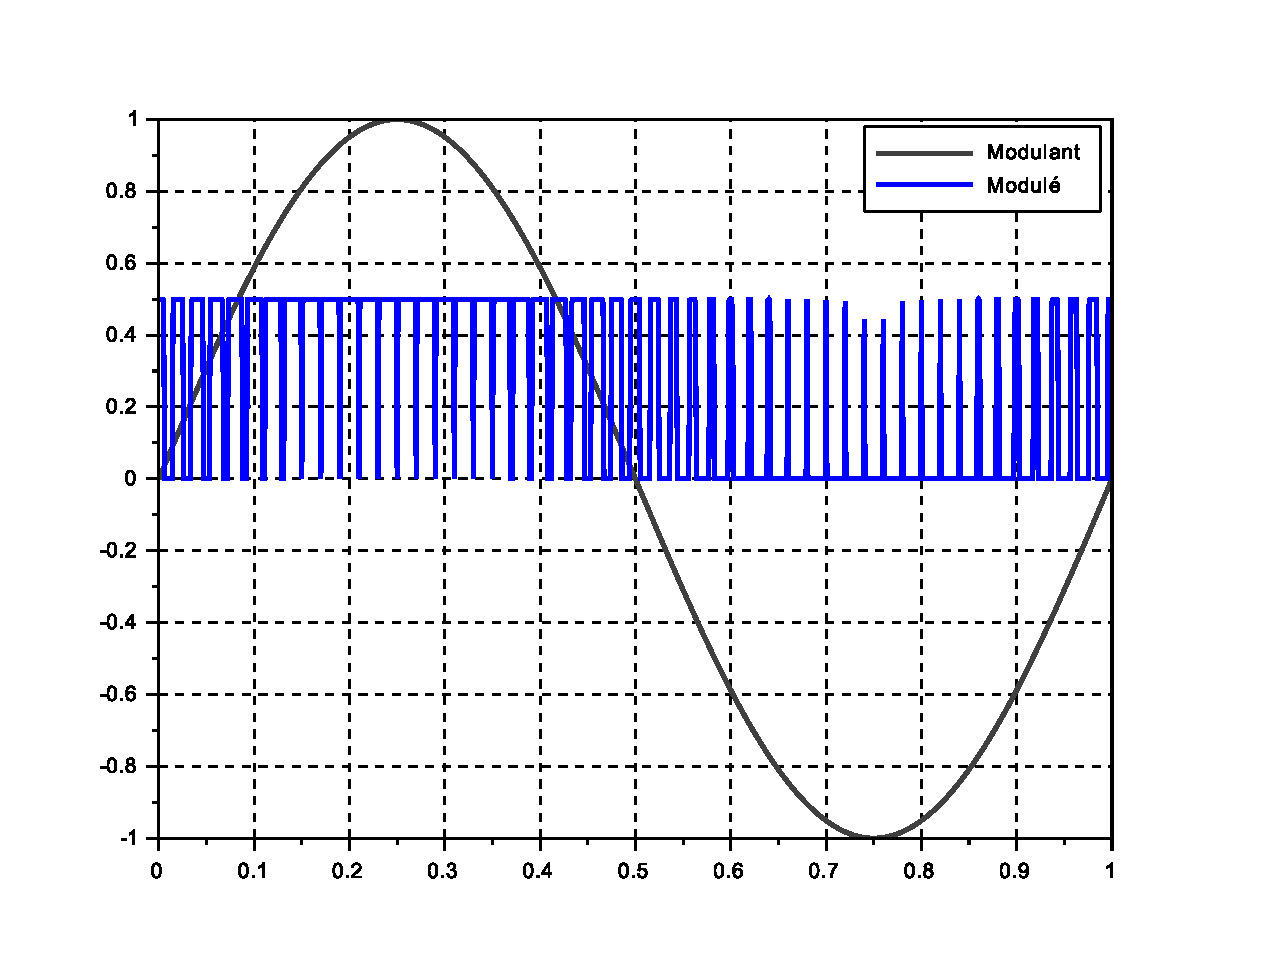
\includegraphics[width=0.8\linewidth]{img/Simu30}
\end{center}
\end{minipage}\hfill
\begin{minipage}{0.48\linewidth}
\begin{center}
 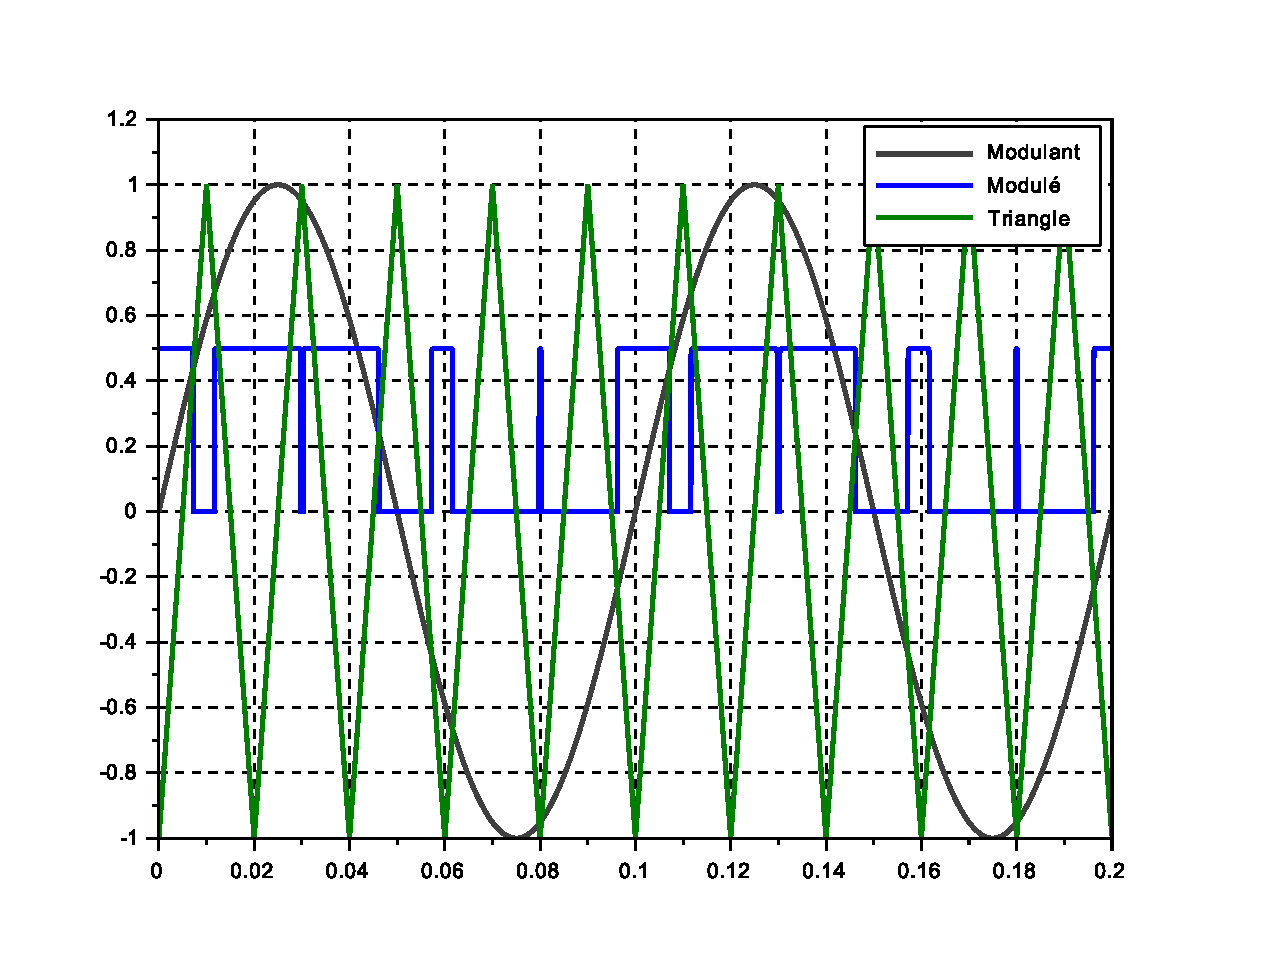
\includegraphics[width=0.8\linewidth]{img/Simu33}
\end{center}
\end{minipage}

Le modulé est défini à partir de la comparaison du modulant et d'un signal triangulaire de même amplitude. \\
\begin{itemize}
 \item Modulant \textbf{au dessus}: le \textbf{modulé vaut 1},
 \item Modulant \textbf{en dessous}: le \textbf{modulé vaut 0},
\end{itemize}

}}

{\frame{
\frametitle{Onduleur}

La charge est donc alimentée par ce montage.

\begin{minipage}{0.48\linewidth}
\begin{center}
 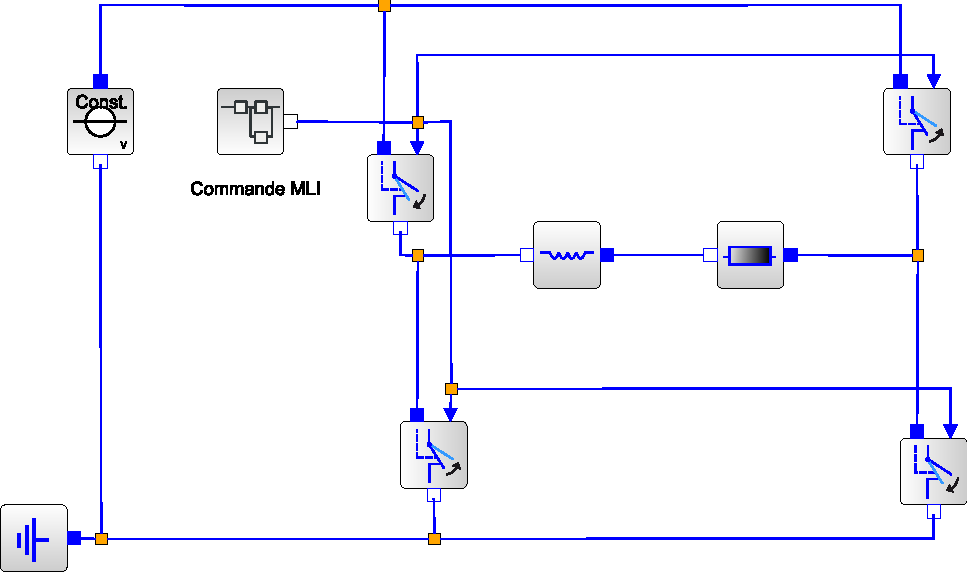
\includegraphics[width=0.8\linewidth]{img/Simu_s04_1}
\end{center}
\end{minipage}\hfill
\begin{minipage}{0.48\linewidth}
\begin{center}
 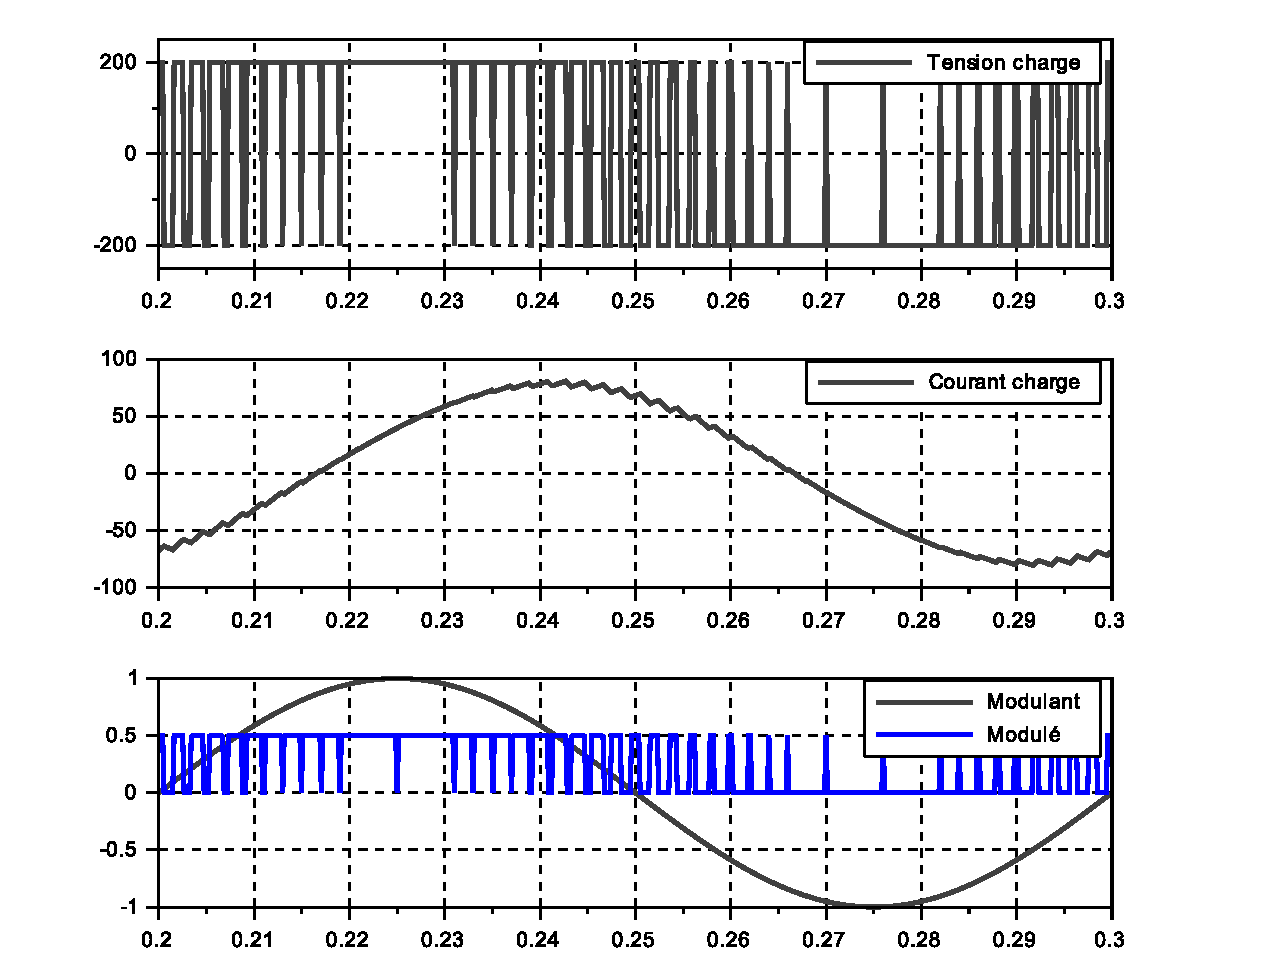
\includegraphics[width=0.8\linewidth]{img/Simu31}
\end{center}
\end{minipage}

On constate alors que:
\begin{itemize}
 \item la forme de la \textbf{tension} est la même que celle du signal modulé,
 \item la forme du \textbf{courant} est lissée par la bobine.
\end{itemize}

}}

{\frame{
\frametitle{Onduleur triphasé}

\begin{wrapfigure}[3]{r}{2cm}
\vspace{-7mm}
\centering 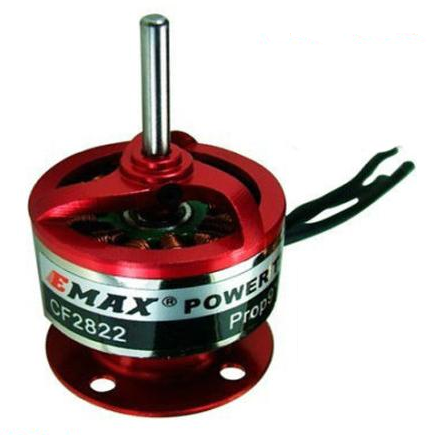
\includegraphics[width=\linewidth]{img/brushless}
\end{wrapfigure}
Un onduleur triphasé peut être utilisé pour l'alimentation d'un moteur triphasé, comme le moteur brushless, très utilisé en modélisme.

Chaque entrée du moteur est connectée à une source de tension, ces phases étant déphasées de $\varphi=\dfrac{2\pi}{3}$.

~\

\centering\begin{circuitikz}[scale=0.5]
\ctikzset{bipoles/length=0.8cm}
\node(0) at (14,4)[color=bleuf,shape=circle,draw] {\Huge{M}};
\draw[color=bleuf] (2,6) node[nigbt, scale=0.5] (npn) {}
 (npn.base) node[anchor=east] {}
 (npn.collector) node[anchor=south] {}
 (npn.emitter) node[anchor=north] {};
 \draw[color=bleuf] (2,2) node[nigbt, scale=0.5] (npn2) {}
 (npn2.base) node[anchor=east] {}
 (npn2.collector) node[anchor=south] {}
 (npn2.emitter) node[anchor=north] {};
 \draw[color=bleuf] (6,6) node[nigbt, scale=0.5] (npn3) {}
 (npn3.base) node[anchor=east] {}
 (npn3.collector) node[anchor=south] {}
 (npn3.emitter) node[anchor=north] {};
 \draw[color=bleuf] (6,2) node[nigbt, scale=0.5] (npn4) {}
 (npn4.base) node[anchor=east] {}
 (npn4.collector) node[anchor=south] {}
 (npn4.emitter) node[anchor=north] {};
  \draw[color=bleuf] (10,6) node[nigbt, scale=0.5] (npn5) {}
 (npn3.base) node[anchor=east] {}
 (npn3.collector) node[anchor=south] {}
 (npn3.emitter) node[anchor=north] {};
 \draw[color=bleuf] (10,2) node[nigbt, scale=0.5] (npn6) {}
 (npn4.base) node[anchor=east] {}
 (npn4.collector) node[anchor=south] {}
 (npn4.emitter) node[anchor=north] {};
 \draw[color=bleuf] (2,0) -- (0,0)  to[V=$U_{in}$] (0,8) -- (2,8);
 \draw[color=bleuf] (10.5,0) -- (2,0);
 \draw[color=bleuf] (2,8) -- (10.5,8) ;
 \draw[color=bleuf] (2,1) -- (npn2.emitter)  (npn2.collector) -- (2,3);
 \draw[color=bleuf] (2,5) -- (npn.emitter) (npn.collector) -- (2,7);
 \draw[color=bleuf] (6,1) -- (npn4.emitter)  (npn4.collector) -- (6,3) ;
 \draw[color=bleuf] (6,5) -- (npn3.emitter) (npn3.collector) -- (6,7);
 \draw[color=bleuf] (10,1) -- (npn6.emitter)  (npn6.collector) -- (10,3) ;
 \draw[color=bleuf] (10,5) -- (npn5.emitter) (npn5.collector) -- (10,7);
 \draw[color=bleuf] (3,1) to[Do] (3,3) ;
 \draw[color=bleuf] (3,5) to[Do] (3,7) ;
 \draw[color=bleuf] (7,1) to[Do] (7,3) ;
 \draw[color=bleuf] (7,5) to[Do] (7,7) ;
 \draw[color=bleuf] (11,1) to[Do] (11,3) ;
 \draw[color=bleuf] (11,5) to[Do] (11,7) ;
 \draw[color=bleuf] (2,1) -- (3,1) (2.5,0)--(2.5,1) ;
 \draw[color=bleuf] (2,5) -- (3,5) (2.5,4)--(2.5,5) ;
 \draw[color=bleuf] (6,1) -- (7,1) (6.5,0)--(6.5,1) ;
 \draw[color=bleuf] (6,5) -- (7,5) (6.5,4)--(6.5,5) ;
 \draw[color=bleuf] (2,3) -- (3,3) (2.5,3)--(2.5,4) ;
 \draw[color=bleuf] (2,7) -- (3,7) (2.5,7)--(2.5,8) ;
 \draw[color=bleuf] (6,3) -- (7,3) (6.5,3)--(6.5,4) ;
 \draw[color=bleuf] (6,7) -- (7,7) (6.5,7)--(6.5,8) ;
 \draw[color=bleuf] (10,3) -- (11,3) (10.5,3)--(10.5,4) ;
 \draw[color=bleuf] (10,7) -- (11,7) (10.5,7)--(10.5,8) ;
 \draw[color=bleuf] (10,1) -- (11,1) (10.5,0)--(10.5,1) ;
 \draw[color=bleuf] (10,5) -- (11,5) (10.5,5)--(10.5,4) ;
 \draw[color=bleuf] (2.5,4.5) -- (12.5,4.5) -- (0) ;
 \draw[color=bleuf] (6.5,4) -- (12.5,4) -- (0) ;
 \draw[color=bleuf] (10.5,3.5) -- (12.5,3.5) -- (0) ;
 \fill (2.5,4.5) circle[color=bleuf,radius=2pt];
 \fill (6.5,4) circle[color=bleuf,radius=2pt];
 \fill (10.5,3.5) circle[color=bleuf,radius=2pt];
\end{circuitikz}
}}

{\frame{
\frametitle{Onduleur triphasé}

La mesure de la \textbf{tension} et du \textbf{courant} dans chacune des bobines d'un moteur alimenté par un \textbf{onduleur triphasé} est présentée ici.

\begin{minipage}{0.48\linewidth}
\begin{center}
 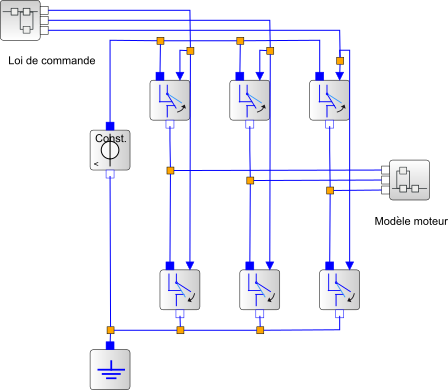
\includegraphics[width=\linewidth]{img/Simu_s04_2}
\end{center}
\end{minipage}\hfill
\begin{minipage}{0.48\linewidth}
\begin{center}
 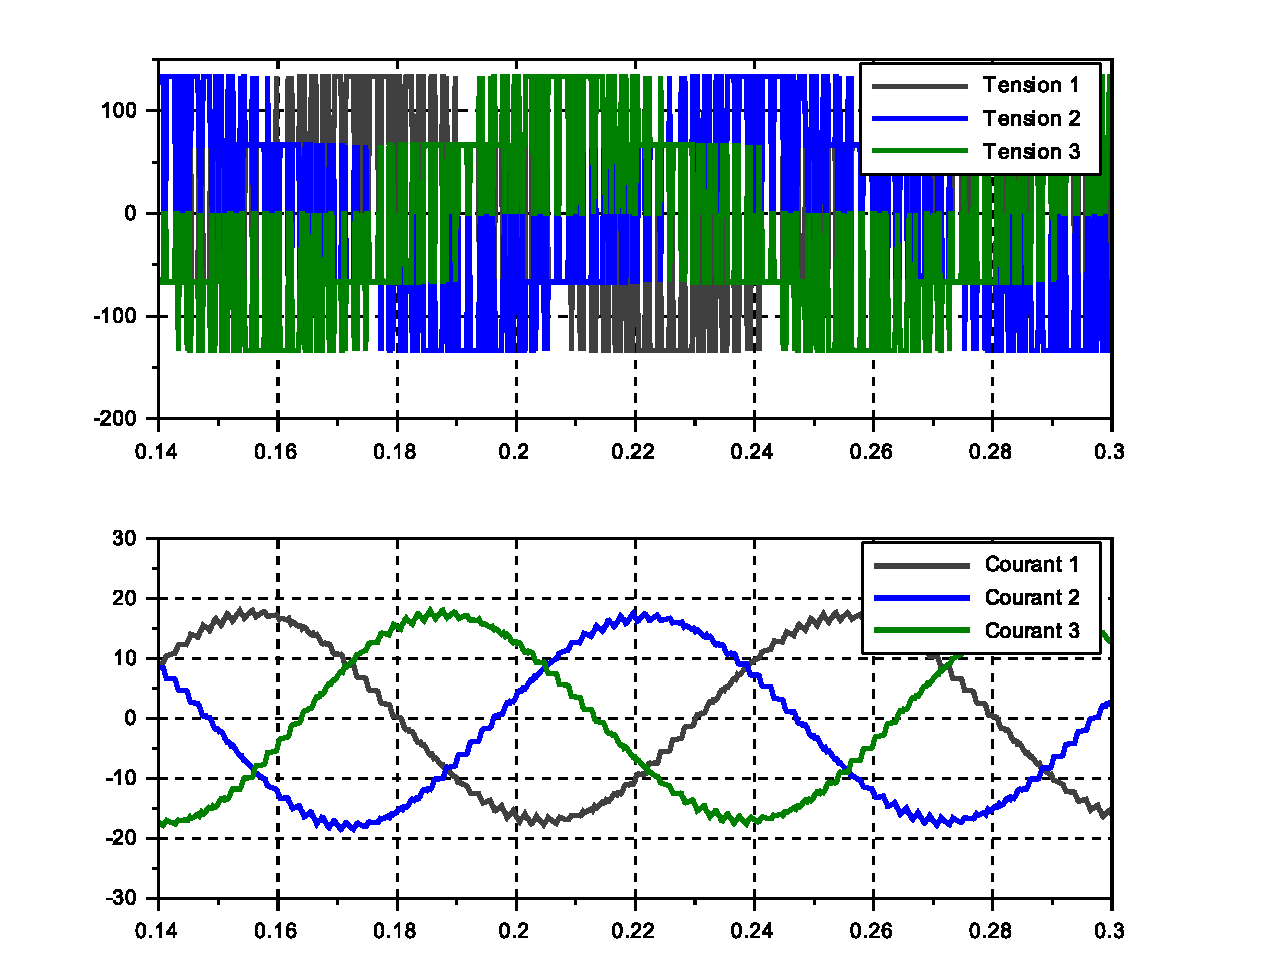
\includegraphics[width=\linewidth]{img/Simu32}
\end{center}
\end{minipage}

Les formes des tensions et courants correspondent à celles présentées précédemment.

}}

{\frame{
\frametitle{Électronique de puissance}

\begin{savoir}
Vous devez être capables :
\begin{itemize}
 \item de modéliser le comportement d'un semi-conducteur,
 \item de modéliser le comportement d'une cellule de commutation,
 \item de concevoir et de commander une cellule de commutation afin de piloter une machine électrique.
\end{itemize}
\end{savoir}

\begin{prob}

Il est nécessaire d'utiliser d'autres formes de représentation d'un mécanisme.
\begin{itemize}
 \item \textit{Problème: Comment modéliser un moteur électrique ?}
 \item \textbf{Perspectives}: Concevoir une chaîne d'énergie électrique en associant une cellule de commutation à la machine électrique correspondante.
\end{itemize}
\end{prob}

}}

\end{document}